\chapter{Query Optimization for Approximate Processing of Time-Travel Queries}
\label{chap:selection}

\section{Introduction}
\label{sec:intro}
\subsection{Motivation and Problem Statement}

 Text search is an expensive operation on web archives due to their large scale. However, many of the documents in the archive contain redundant information. In certain scenarios, users are often satisfied with a subset of the true results that are determined \emph{quickly}. That is, missing a few results during search might not lead to substantial information loss. Particularly in search tasks which involve multiple interactive steps of query reformulation, expansion, and refinement. Consider the following two use cases in the context of time-travel text search. 

\begin{itemize}

  \item A sports journalist is in interested the game between the popular cricket teams, from Mumbai and Rajasthan, and issues a query \query{indians vs royals}{6/2008}. However content from the popular baseball teams from Cleveland and Kansas, also having the same titles, which also were in the news in the same period might dilute the results. For an interactive and constructive search experience the analyst should be able to quickly identify the ambiguity of the keywords used and alter the query to \query{mumbai indians vs rajasthan royals}{6/2008}. Here a subset of the exact results is good enough for the user to adapt \kwquery{indians vs royals} to \kwquery{mumbai indians vs rajasthan royals}. 

  \item  Partial results can also help reformulating for the correct temporal predicates of the query. Consider the utility of time-travel text search in patent retrieval. The time-interval of a query \query{retina display patent}{1/2010 - 12/2012} can quickly be reformulated to \query{retina display patent}{6/2012 - 6/2013} when the user observes that the initial results cluster around the second half of the year 2012. 

\end{itemize}

In such scenarios, a subset of the results is often representative of the information contained in the entire result set. Increasing the number of elements in this subset, or the recall, improves the information contained therein. Also, it is imperative that the user needs to have the ability to control the performance of the time-travel retrieval task. To this extent, we develop query processing techniques to maximize recall, for a time-travel query, given a user-specified bound on the performance.

%\aanand{Consistency issues: partial results vs. subset of results...}

\subsection{Approach}
In the previous chapters we discussed different index-organization strategies for web archives with the focus on \emph{exact} solutions to time-travel queries. 
%We established that for exact results to time-travel queries, horizontal partitioning was a desirable index organization strategy. 
We showed that horizontal partitioning is an efficient index-organization strategy for exact time-travel queries. In this chapter, we argue that, for approximate processing of time-travel queries vertical partitioning is more suitable. This is due to the fact that vertical partitions are clustered in the time dimension. 

By identifying the time periods which have high result contribution, and in turn the partitions which temporally overlap with it, the recall can be increased by processing such partitions early on.
%We can increase the partial result size by identifying time-periods where results are clustered. The partitions corresponding to these time-periods are processed early.
%Large number of results can be computed by identifying time-periods where the results are clustered by processing the partitions that overlap with it temporally. 
In contrast, a lack of such clustering in horizontal partitioning or sharding prevents easy identification of shards which have high result contribution.
%This is unlike horizontal partitioning where a lack of temporal clustering prevents easy identification of shards for partial result computation. 
Consequently, we operate on an index with vertically-partitioned posting lists and propose query-optimization methods to determine partial results efficiently.
%and augment the query processor with a query-optimizer for determining quick partial results. 

%challenges and design decisions
A natural side effect of vertical partitioning is that postings with long valid-time intervals are replicated across several temporally-adjacent partitions. This is not an issue for time-point queries where only one partition per term is accessed during query processing. For the more practical and general class of time-travel (text) queries where the temporal predicate is a \emph{time interval}, the straightforward query processing of~\cite{kberberi:sigir2007} quickly becomes inefficient as a consequence of this replication, as repeatedly reading replicated postings from several partitions within the query time-interval wastes I/O operations. 


%\subsection{Selecting Partitions for Query Processing}
We introduce an approach called \emph{partition selection} which  exploits the following observation: %in a temporally partitioned index, 
if we can determine that a partition largely consists of postings that are replicated in
already processed partition(s), we can avoid processing this
partition without significantly compromising the final result
quality. 
We aim at \textit{selecting a set of partitions} which can be processed
incurring no more than a given maximal processing cost and 
that yield high recall.
%RJS: needs to be refined
We consider abstract
cost measures for processing a query, namely
the number of partitions or the number of postings 
accessed during execution. A user would specify bounds
on the execution time that can be transformed into bounds on the abstract
cost by the system. Alternatively, the user can also stop the processing
at any time when she determines that the results are already satisfying
(or the query needs to be refined); our methods support this
by selecting partitions first that are likely to contain many unseen answers.

We use the example in Figure~\ref{fig:intro_example} to
illustrate the general idea of our approach. This figure shows posting lists for two terms \textsc{A} and \textsc{B}
built over documents with valid-time intervals. On
the left side of the figure, posting lists are shown, each spanning
the entire time interval. %lifetime of their corresponding term. 
The region, shaded in gray, represents a temporal predicate that spans a small time
range over these lists. In the absence of temporal partitioning, 
query processing needs to entirely scan both lists and
filter out postings that do not satisfy the temporal
predicate. When the index is partitioned, however, the processing can
be sped up by reading only the relevant partitions that overlap with
the temporal predicate, represented on the right. Thus, in our example, a total of 6 partitions -- $A_1, A_2,
A_3$ and $B_1, B_2, B_3$ -- have to be processed to determine the
result set of $\{d_1, d_2, d_3\}$ -- marked as red line-segments.


\label{subsec:contributions}

  \begin{figure}[tb]
  \centering
    \includegraphics[width=\columnwidth]{resources/vp_qp.pdf}
  \caption{Processing a time-travel query ``A B" @ [$t_b$ , $t_e$] using partition selection} 
    \label{fig:intro_example}
\end{figure}

However, a closer inspection of Figure~\ref{fig:intro_example} reveals
that the same result set can be obtained by processing only \emph{2
  partitions}, $A_2$ and $B_2$, since the replicas of
postings for documents in the result set are fully available within
these two partitions.

How can we make use of this observation in practice ? In order to do
so, we need to answer the following questions: (i) does a partition contribute non-redundantly towards the
final result set when it is processed ?, (ii) how much does a partition contribute to the final result set ? (iii) is there an alternative set of
partitions which can contribute these answers at a lower access
cost ? Based on answers to these questions, we can generate a partition-access plan so that for a specified cost budget only those
partitions are chosen for processing which maximize the number of
results.

% In this chapter, we address these issues in detail and propose the following problem:

% %\textbf{Problem 1} 
% \textit{Given an upper-bound on the I/O cost incurred during query
% processing, select a subset of partitions so that the
% recall of the final result is maximized without exceeding the
% specified upper-bound.}

\subsection{Contributions}

We formally model these \emph{partition selection} problems as optimization problems. Making use of KMV synopses for cardinality estimation
under set operations~\cite{kmv:sigmod}, we develop algorithms for efficiently
solving such partition-selection problems. In particular, the contributions made in this chapter are:

\begin{enumerate}
\item An optimal dynamic programming based partition selection algorithm for single-keyword queries;

\item An efficient greedy alternative for partition selection that can
  be applied for both single keyword as well as multi-keyword queries;

\item A detailed experimental evaluation on three large-scale real-world
  text archives: the revision history of the English Wikipedia, a Web archive, and the
  Annotated New York Times archive spanning 20 years.
\end{enumerate}

\subsection{Organization}
The remainder of this chapter is organized as follows: in Section~\ref{chap:selection:sec:model}, we present index organization and query processing in our setup. In Section~\ref{sec:singleterm-selection}, we detail an optimal algorithm and
its greedy approximation for selecting the set of partitions to process for
the case of single-keyword queries. Extensions for multi-term query
setting are described in Section~\ref{sec:psmtq}. Our experimental setup and results are detailed in Section~\ref{chap:selection:sec:evaluation} before summarizing in Section~\ref{chap:selection:sec:summary}. 


\section{Index Organization and Query Processing}
\label{chap:selection:sec:model} 

We adopt the document, collection and query models from the previous chapters (c.f. Section~\ref{chap:sharding:sec:model} and Section~\ref{chap:foundations:sec:model}). We briefly recap the notation in Table~\ref{tab:selection_notation}.

\begin{table}
\centering
\begin{tabular}{ll}
\hline  
\multicolumn{1}{l}{\emph{Notation}} &  \multicolumn{1}{l}{\emph{Description}} \\
\hline
$\mathcal{D}$ & collection of documents\\
$\mathcal{V}$ & \emph{vocabulary} as a set of words\\
$d_i^j \in \mathcal{D}$ & the $j^{th}$ version of document $d_i$\\
$valid(d_i^j)$ & valid-time interval \\ 
$begin(d_i^j)$ & begin-time of $d_i^j$  \\
$end(d_i^j)$ & end-time of $d_i^j$ \\
$Q$ & time-travel query\\
$keywords(Q)$ & set of keywords in $Q$\\
$interval(Q)$ & query time-interval of $Q$\\
$I_1 \overlaps I_2$ & Overlapping intervals $I_1$ and $I_2$ \\
$I_1 \noverlaps I_2$ & Non-overlapping intervals $I_1$ and $I_2$ \\
\hline
\end{tabular}
\caption{Notation.}
\label{tab:selection_notation}
\end{table}

\paragraph{Index Organization}

We use a temporally-partitioned index as described in Chapter~\ref{chap:foundations} with the following posting structure 
$$
  \langle d_i^k, [begin(d_i^{k}), end(d_i^{k}))\rangle.
$$

 $d_i^k$ refers to the version identifier $d_i^{k}$, $[begin(d_i^{k}), end(d_i^{k}))$ is its valid-time interval.

The temporally-partitioned index consists of posting lists vertically partitioned into a set of partitions. We let $partitions(v)$ denote the set of partitions of the posting list $L_v$ for term $v \in \mathcal{V}$. Each partition $\slice_{v,j} \in partitions(v)$ has an associated time-interval $span(\slice_{v,j}) = [begin(\slice_{v,j})\,,\, end(\slice_{v,j}))$ and stores postings representing document versions whose valid-time intervals overlap with $span(\slice_{v,j}) $, i.e.,

\begin{equation*}
  \slice_{v,j} = \bigset{ \, d_i^k \in \mathcal{D} \:\:|\:\: v \in d_i^k \:\wedge\: valid(d_i^k) \overlaps span(\slice_{v,j})\,} \;.
\end{equation*}

Further, we assume that partition spans for a given term $v$ are disjoint, i.e.,
\begin{equation*}
  \forall{i}\:\:\forall{j}\::\: span(\slice_{v,i})\,\, \noverlaps \,\,span(\slice_{v,j})\;.
\end{equation*}

A lexicon $\mathcal{L}$ stores this partitioning information as a mapping from term to the partition statistics (partition span, partition size and location).

For a pair of partitions $\slice_{v,i}$ and $\slice_{v,i+k}$, or simply $\slice_{i}$ and $\slice_{i+k}$, $\slice_{i} \cap \slice_{i+k}$ represents the set of postings common to both the partitions. The overlap of valid-time intervals and partition spans gives rise to the time-continuity property as described below. 
\begin {lemma}[Continuity Property in Vertical Partitions]
  \label{lem:eff}
  For a set of partitions belonging to a term $v$, the overlaps of contents of partition $\slice_{i}$ with
  $\slice_{i+k}$, $\forall k \geq 0$ and $0 \leq j \leq k$ have the following property:
$$
  \slice_{i} \cap \slice_{i+k} \subseteq \slice_{i} \cap \slice_{i+j}
$$
\end{lemma}
\begin{proof}{}
  Every posting $p \in \slice_{i} \cap \slice_{i+k}$ represents a version $d_k^t $ for which $begin(d_k^t) < end(\slice_i)$ and $end(d_k^t) > begin(\slice_{i+k})$. This implies that 
  $$
    valid(d_k^t) \overlaps span(\slice_{i+k} )
  $$
   and hence the claim holds.
\end{proof}

% Each index-list is partitioned along the time-axis into vertical partitions

% and each partition is associated with a time-interval . 

% In detail, we let $\slice_v$ denote the set of
% partitions of the inverted list $L_v$ for term $ v \in \mathcal{V}$. Every partition $\slice_{v,j}$ has an associated time interval
% $[b_{v,j},\,e_{v,j})$ and contains (identifiers of) all documents in $L_v$ that
% existed at any time during the time interval associated with $\slice_v$, i.e.,




\paragraph{Query Processing}
In this work we use conjunctive query semantics, i.e., we identify as results documents versions that contain all query terms. We employ the Term-at-a-Time (\textsc{TaaT}) approach of posting-list intersection during query processing. First, the partitions overlapping with the query time-interval are determined by consulting the lexicon. We refer to these partitions as \emph{affected partitions}. 
%We firstly determine the term-partitions, referred to as affected partitions, which overlap with the query time-interval by looking up the lexicon. 

\begin{definition}[Affected Partitions]
For a time-travel query Q, the set of partitions of the term $q_i \in keywords(Q)$ which overlap with the query-time interval $interval(Q)$ are 
$$ a(q_i, Q) \,= \, \bigset{  \slice_{i,j} \,\,\, | \,\,\, interval(Q) \overlaps span(\slice_{i,j})}. 
$$
\end{definition}
When it is clear from the context we use $a_i$ for $a(q_i, Q)$. The overall set of affected partitions is $A(Q) = \bigcup_{q_i \in keywords(Q)} a_i$. The determined $a_i$s are merged to determine a candidate set of postings which overlap with $interval(Q)$. Following that, these candidate sets are intersected employing \textsc{TaaT} posting-list intersection, for the final set of results.
%\aanand{do we need an example from the figure here ? For now I'll pass.}

For approximate processing of time-travel queries we additionally go through a query-optimization phase prior to query processing -  referred to as \emph{partition selection}. Partition selection determines a subset $\mathcal{S} \subseteq A(Q)$ of all the affected partitions for query processing. Query processing over $\mathcal{S}$ yields partial results. We formalize the notion of a result set $R(\mathcal{S},Q)$ given a time-travel query $Q$ over a subset of affected partitions $\mathcal{S} \subseteq A(Q)$.

\begin{equation}
R(\mathcal{S},Q) \!=\!
\left\{\begin{array}{c@{\,:\,\,}c}
 \bigset{ \,\,\bigcup_{\slice_j \in \mathcal{S}}{\slice_{j}} \,\,}& |Q| = 1\\
 \bigset{ \,\,\bigcap_{1 \leq i \leq |Q|}\,\bigcup_{\slice_{i,j} \in \mathcal{S}}{\slice_{i,j}} \,\,} & |Q| > 1.
 \end{array}\right.
\end{equation}

Using the notation above, the exact set of results is captured hence by $R(A(Q), Q)$. The case when $|Q| = 1$ refers to the scenario when the query contains a single keyword. In such a case all postings accessed are relevant and are captured by the union operation over all affected partitions. However, when $|Q| > 1$, only those postings which are common to all the terms are relevant. This is captured by the intersection over unions. As an example, we refer to Figure~\ref{fig:intro_example}. For a query \query{A B}{$t_b$, $t_e$} the document versions, colored in red, are retrieved as results. However, for a single-term query, say \query{A}{$t_b$, $t_e$}, all document versions index in ``A'' get qualify as results.

To quantify how much of the exact results are retrieved using $\mathcal{S}$ we use relative recall. The relative recall for $\mathcal{S} \subseteq A(Q)$, $RR(\mathcal{S},Q)$, is defined as the ratio of the number of retrieved results to that of the exact results, i.e., fraction of results retrieved. Formally, 

\begin{equation}
RR(\mathcal{S},Q) \!=\! |R(\mathcal{S},Q)| / |R(A(Q),Q)|.
\end{equation}

The intention of partition selection is to choose $\mathcal{S}$ in order to maximize $RR(\mathcal{S},Q)$.

\paragraph{Use of Partition Synopsis}
Partition-selection algorithms, as we discuss in detail later, use cardinality values of set operations (unions and intersections) on partitions as primitive operations. However, to determine the exact cardinalities the partitions have to be accessed which is exactly what we want to avoid. Instead, we depend on high quality cardinality estimates under union and intersection of large sets of document identifiers. For this purpose, we utilize the recently proposed KMV synopses~\cite{kmv:sigmod}. In a pre-computation step, we build and store the synopsis for each partition on disk of the temporally-partitioned index, which we use during our partition-selection process. Pointers to each partition-synopsis can be either stored in the existing lexicon or an altogether separate lexicon can be constructed explicitly for this task.

During partition selection, the lexicon storing pointers to partition synopses is consulted followed by retrieval of the synopsis of each affected partition. These highly compact partition synopses are used by our selection algorithms to determine cardinalities of set operations over partitions. In the next section, we first detail partition-selection methods for queries with only single terms. We then generalize these approaches to multi-term queries.

\section{Single-Term Partition Selection}
\label{sec:singleterm-selection}

Let us consider the special case where the time-travel keyword query
$Q$ consists of only a single query term, i.e., $keywords(Q) =
\{\,q\,\}$. Since we deal with single-term queries, we denote $\slice_{q,j}$ as $\slice_{j}$ for ease of notation from now on. 

Our objective, when selecting partitions to process the
time-travel keyword query, is to retrieve as many of the original query
results as possible, while not violating a user-specified I/O
bound. Our optimization objective, to put it differently, is to
maximize the \textit{relative recall} as the fraction of original query
results retrieved. The user-specified I/O bound, which constrains the
space of valid solutions, can be of two types -- \textit{size-based partition selection} or \textit{equi-cost partition selection}. 

In both selection problems we model the performance to be proportional to the index accesses. Hence a bound on the accesses simulates a bound on the response time for a time-travel query. In case of \textit{size-based partition selection} we bound the number of postings accessed. A similar analysis is undertaken for most query-processing methods over posting lists.

However, we also take a more coarse-grained approach in modelling the constraint on accesses in \textit{equi-cost partition selection}. Accesses to each partition results in a random access and random I/O are substantially more expensive than sequential I/O. Also, partitions tend to be smaller than entire posting lists. Hence the bottleneck in answering a time-travel query in such scenarios is the number of distinct partitions that are accessed. To this extent, in \textit{equi-cost partition selection}, we model the allowable budget to be accessed as a fixed number of affected partitions that can be accessed rather than number of postings.

%\subsection{{Entry-Based Partition Selection}}
\paragraph{Size-Based Partition Selection}
\label{sec:ebps}
The input to this optimization problem is the set of affected
partitions $A(Q)$, and a
user-specified I/O bound $\beta$ where $0 < \beta \leq 1$. Here, $\beta$ denotes the fraction of postings of all affected partitions that we are allowed to read. The cardinality of each partition $|\slice_j|$ represents the number of postings accessed on selecting the $|\slice_j|$ for processing. Note that maximizing result size $\big\vert \bigcup_{\slice_j \in \mathcal{S}}{\slice_{j}} \big\vert$ is equivalent to maximizing relative recall since the original result size $\big\vert \bigcup_{\slice_j \in A(Q) }{\slice_{j}} \big\vert$ is constant. Thus, we intend to determine $\mathcal{S} \subseteq A(Q)$ so as to maximize the result size while retaining our I/O budget. Formally, 
% \begin{definition}[Relative Recall]
% Relative recall or simply recall for any $\mathcal{S} \subseteq \slice$ for single-term partition selection, is defined as

% $$
%   r(\mathcal{S}) = \frac{\big\vert \bigcup_{\slice_j \in \mathcal{S}}{\slice_{j}} \big\vert}{\big\vert \bigcup_{\slice_j \in \slice }{\slice_{j}} \big\vert}.
% $$
% \end{definition}


\begin{definition}[Size-Based Selection for Single-Term Queries]
\label{def:sbs_sts}
\begin{equation*}
  \argmax{\mathcal{S} \subseteq \slice}{\left| \bigcup_{\slice_j \in \mathcal{S}}{\slice_{j}} \right|} \quad \mbox {s.t.}  
\end{equation*}
\begin{equation*}
  \sum_{\slice_j \in \mathcal{S}} |\slice_{j}| \,\,\,\leq \,\,\,\beta \cdot \left(\sum_{\slice_i \in A(Q)}|\slice_{i}|\right).  
\end{equation*}
\end{definition}



% \begin{definition}[Size-based Partition Selection Problem]

% \begin{equation*}
%   maximize \,\, \big\vert \bigcup_{j, x_{j} \neq 0}{\slice_{j}} \big\vert \quad \mbox{s.t.}  
% \end{equation*}
% \begin{equation*}
%   \sum_{j} x_{j} \cdot |\slice_{j}| \,\,\,\leq \,\,\,\beta \cdot (\sum_{j}
%   |\slice_{j}|)  
% \end{equation*}
% \begin{equation*}
%   x_{j} \in \{0,1\}\;.  
% \end{equation*}

% where $x_j$ is an indicator variable which denotes whether the
% partition $\slice_{j}$ is selected.
% \end{definition}

\paragraph{Equi-Cost Partition Selection}
\label{sec:pbps}
The inputs to this problem is the same as before -- $\slice_{j}$, and bound ${\beta}$. However, we assume that all partitions are equally expensive to process irrespective of their sizes. The constraint is now bound to a fixed number of partitions that can be accessed $\beta\cdot|\slice|$. The objective function remains the same as before. Formally,

% \begin{definition}[Equi-cost Partition Selection Problem]
% $$
% maximize \,\, \big\vert\bigcup_{j, x_{j} \neq 0}{\slice_{j}} \big\vert \quad \mbox{s.t.}
% $$
% $$
% \sum_{j} x_{j} \,\,\,\leq \,\,\, \beta \cdot N
% $$
% $$
% x_{j} \in \{0,1\}.
% $$

% \end{definition}

\begin{definition}[Equi-Cost Selection for Single-Term Queries]

\begin{equation*}
  \argmax{\mathcal{S} \subseteq \slice}{\left| \bigcup_{\slice_j \in \mathcal{S}}{\slice_{j}} \right|} \quad \mbox {s.t.}  
\end{equation*}
\begin{equation*}
  |\mathcal{S}| \,\,\,\leq \,\,\,\beta \cdot \left|A(Q) \right|.  
\end{equation*}
\end{definition}

%It can be observed that this is a special case of the size-based partition selection problem defined above, obtained by setting the value of $1$ as the cost of each partition. 

\subsection{Optimal Algorithm for Single-Term Partition Selection}

The above problems can be solved using dynamic programming over an
increasing number of affected partitions. We first present a solution to the more general size-based partition selection. Our solution to equi-cost partition selection follows from this, as we show later. 

We process the affected partitions $A(Q)$ in the order of their begin times, i.e., $$begin(\slice_{v,j}) < begin(\slice_{v,j+1}).$$ Consider a prefix sub problem which considers affected partitions $\{\slice_{1}, \cdots, \slice_{k} \} $, and capacity $c = \beta \cdot (\sum_{j}|\slice_{j}|) $. Let $\textsc{Opt}(c,k)$ denote the optimal set of partitions for the prefix sub-problem with capacity $c$, the optimal result-set size hence is $R(\textsc{Opt}(c,k))$. The optimal solution is computed by the following recurrence on the constituent sub-problems. 

%$r(\mathcal{S}_{c,k})$ denote the recall of the optimal solution $\mathcal{S}_{c,k}$ to the sub-problem. The recurrence relation for computing $r(S_{c,k})$ using sub-problems $\mathcal{S}_{c',k'}$ ($0 \leq c' \leq c$ for integral values of c') is:

\begin{equation*}
R\,\left(\,\textsc{Opt}(c,k)\,\right) \!=\! \,\,\, max
\left\{\begin{array}{c@{\,\,\,}c}
 R\, \left(\,\textsc{Opt}(c,k-1)\,\right)\\
 \!\!\simplemax{\,0 < k' < k}{  R\,\left(\,\,\textsc{Opt}\left(c-|\slice_{k}|\,\,,\,\,k'\,\,\right)\,\,
  \, \bigcup \,\,\,\{\slice_{k}\} \,\,\right)} 
 \end{array}\right.
\end{equation*}

We now state and prove the optimality of the recurrence in Theorem~\ref{thm:epbs}.

\begin{theorem}
  \label{thm:epbs}
     Given a query $Q$ and access budget of capacity $c = \beta \cdot (\sum_{\slice_j \in A(Q)}\,\,|\slice_{j}|)$ the optimal solution to the size-based selection problem is given by $\textsc{Opt}(c,|A(Q)|)$. 
\end{theorem}

\begin{proof}{}
  % \newline
Assume that we have optimal solutions for all sub-problems by the given recurrence, $\textsc{Opt}(c',k')$, with capacities $c'$ such that $0 < c' < c$, for the set of partitions $\{ \slice_{i} \}$ where $$0 < k' < k.$$ Now we consider computing the optimal selection set by the recurrence $\textsc{Opt}(c,k)$ using $\textsc{Opt}(c',k')$'s. Let us assume that there is a better solution $\overline{\textsc{Opt}}(c,k)$ such that 
$$R(\overline{\textsc{Opt}}(c,k)) > R(\textsc{Opt}(c,k)).$$

  {\bf Case 1 -- $\slice_k \notin \textsc{Opt}(c,k)$ :} From the recurrence this means $$R(\overline{\textsc{Opt}}(c,k)) > R(\textsc{Opt}(c,k-1))$$ since
  $R(\textsc{Opt}(c,k)) = R(\textsc{Opt}(c,k-1))$ when $\slice_k \notin \textsc{Opt}(c,k)$. As a consequence, we have a new
  optimal solution for the sub-problem for capacity $c$ and the set of
  partitions $\{ \slice_{i}\}$ where $0<i<k$, i.e, $R(\overline{\textsc{Opt}}(c,k-1)) > R(\textsc{Opt}(c,k-1))$. But, this is contrary to our initial assumption since we assumed $R(\textsc{Opt}(c,k-1))$ is optimal for $\{ \slice_{i}\}$ where $0<i<k$. Thus, by contradiction our claim holds.

  {\bf Case 2 -- $\slice_k \in \textsc{Opt}(c,k)$ :} The second relation in the recurrence is applicable now. Our assumption leads to the condition $R(\overline{\textsc{Opt}}(c,k)) >
  \simplemax{\,0 < k' < k}{  R\,\left(\,\,\textsc{Opt}\left(c-|\slice_{k}|\,\,,\,\,k'\,\,\right)\,\,
  \, \bigcup \,\,\,\{\slice_{k}\} \,\,\right)}$. 

  Let us denote the index of the partition selected just before $\slice_{k}$ for $\overline{\textsc{Opt}}(c,k)$ to be $k'$, i.e., for $k' = \argmax{}{\overline{\textsc{Opt}}(c,k) \backslash \{\slice_{k}\}}$. According to our assumption we have 
\begin{eqnarray*}
  R(\overline{\textsc{Opt}}(c,k)) - \left|\slice_{k} \cap \slice_{k'} \right| &>& \left(\simplemax{\,0 < k' < k}{R(\textsc{Opt}(c,k))} \right)- \left|\slice_{k} \cap \slice_{k'} \right|\\
  \implies R(\overline{\textsc{Opt}}(c-|\slice_{k}|,k')) &>& R(\textsc{Opt}(c,k')) - \left|\slice_{k} \cap \slice_{k'} \right|\\
  \implies R(\overline{\textsc{Opt}}(c-|\slice_{k}|,k')) &>& R(\textsc{Opt}(c-|\slice_{k}|,k'))
\end{eqnarray*}
  
This is a contradiction since $\textsc{Opt}(c-|\slice_{k}|,k')$ is optimal for all $0 < c' < c$. Hence our claim in the theorem holds true.
  %This is contrary to  and hence by contradiction our claim in the Theorem holds true. 
  \end{proof}

 \begin{algorithm}[htb!]
   \begin{algorithmic}[1]
     \STATE $c_{max}=\,\lfloor \beta \cdot (\sum_{j}
   |\slice_{j}|  \rfloor$ 
   \STATE // Dynamic programming table, $n$ is number of affected partitions
   \STATE $DP\,[\,0\,..\,c_{max}\,][\,0\,..\,n\,]$ \quad 
  \STATE \FOR{$i = 0\,..\,c_{max}$}
     \STATE $DP\,[\,i\,][\,0\,] = \emptyset$
      \ENDFOR
 
  \STATE \FOR{$k = 1\,..\,n$} 
      \FOR{$i = 0\,..\,  |\slice_{k}| - 1$}
         \STATE $DP\,[\,i\,][\,k\,] = \emptyset$\quad // No partitioning possible
      \ENDFOR
     
      \FOR{$i = |\slice_{k}|\,..\,c_{max}$} 
        \FOR{$k' = 0\,..\,k-1$} 
          \STATE // Update if recall is better than current value
          \STATE $r_{k'} = DP_r\,[\, i - |\slice_{k}|\,][\,k'\,] + (|\slice_{k}| - (\slice_{k} \cap DP_{lp}\,[\,i - |\slice_{k}|\,][\,k'\,]))$ 
        \ENDFOR
        \STATE $k' = \argmax{}{r_{k'}}$
        \STATE   // Update the DP table with the best partitioning
            \STATE  $DP_r\,[\,i\,][\,t\,] = max \{ DP_r[c_j][k_i - 1], r_{k'} \}$
        \STATE    $DP_{lp}\,[\,i\,][\,t\,] = \argmax{}{DP_r\,[\,i\,][\,t\,]}$ 
              
          \ENDFOR
        \ENDFOR
      \STATE \STATE {\bf return} $DP[\,c_{max}\,][\,n\,]$ 
   \end{algorithmic}
   \caption{Partition Selection - dynamic programming solution}
   \label{alg:partselect}
 \end{algorithm}

Algorithm~\ref{alg:partselect} efficiently implements the recurrence relation presented above. Each of the \textsc{DP} table cell contains a pair of values -- (i) the last partition selected, $DP_{lp}$, for the corresponding sub-problem (i.e., the selected partition with the maximum begin-time), and (ii) the optimal recall value $DP_r$. Since the choice of partitions cannot be
made independently, the computation of recall for a newly selected
partition takes into account only the postings that are not already
included in previously selected partitions. Using Lemma~\ref{lem:eff},
we can efficiently compute the optimal recall for each sub-problem
since all overlaps with the preceding partitions to $lp$ are already
covered in $lp$. 

 The \textsc{DP}-based algorithm, outlined in Algorithm~\ref{alg:partselect}, has a time complexity $\mathcal{O}(n^2 \cdot (\sum_j |\slice_{j}|))$, where $n$ is the number of affected partitions, and a space
 complexity of $\mathcal{O}(n \cdot (\sum_j |\slice_{j}|))$. The optimal partitioning can be easily computed by backtracking from the best solution seen at $\textsc{DP}_{lp}[\,c_{max}\,][\,n\,]$. Observe that the complexities depends on the cardinalities of the partitions, i.e.,$\sum_j |\slice_{j}|)$. Thus, Algorithm~\ref{alg:partselect} is a pseudo-polynomial algorithm, for size-based partition selection, which is polynomial in the value of the size bound.
 

Equi-cost partition selection is a special case of size-based selection and employs a uniform cost per partition. The recurrence relation for equi-cost selection is 

\begin{equation*}
R\,\left(\,\textsc{Opt}(c,k)\,\right) \!=\! \,\,\, max
\left\{\begin{array}{c@{\,\,\,}c}
 R\, \left(\,\textsc{Opt}(c,k-1)\,\right)\\
 \!\!\simplemax{\,0 < k' < k}{  R\,\left(\,\,\textsc{Opt}\left(c-1\,\,,\,\,k'\,\,\right)\,\,
  \, \bigcup \,\,\,\{\slice_{k}\} \,\,\right)} 
 \end{array}\right.
\end{equation*}
 
 This results in improvements in both the space and time complexity of the algorithm, as the optimal value is independent of the sum of the sizes of the partitions read. The time complexity of the algorithm
reduces to be $\mathcal{O}(n^3)$ and a space complexity of
$\mathcal{O}(n)$. Note that unlike the algorithm for size-based selection, the algorithm for equi-cost selection is a polynomial algorithm which is polynomial in the number of partitions affected.  

\subsection{Approximation Algorithm}
\label{sec:approx}
While the selection algorithms outlined above allow for polynomial run
times, they might not be efficient enough to be applied during query
processing, e.g., when the partitions contain a large number of postings. Alternatively, we propose the use of
$(1-\frac{1}{e})$-approximation algorithm called
\emph{Greedy\-Select}, developed in~\cite{budgetedmaxcover} for solving
\emph{budgeted maximum coverage} (BMC) problem. We first show
the equivalence of our partition selection problem and the BMC
problem.

\begin{definition}[Budgeted Maximum Coverage] A collection of sets $\mathcal{S} = \{ \mathcal{S}_1 , \mathcal{S}_2, \ldots , \mathcal{S}_m\}$ with associated costs $\{ c_i \}$ is defined over a domain of elements $X= \{ x_1,x_2, \ldots,x_n\}$ with associated weights $\{ w_i \}$. The goal is to find a collection of sets $\mathcal{S}' \subseteq \mathcal{S}$, such that the total cost of the elements in $\mathcal{S}'$ does not exceed a given budget L, and the total weight of every element covered by $\mathcal{S}'$ is maximized.

\end{definition}

\begin{lemma}
  Partition selection is an instance of budgeted maximum coverage (BMC).
\end{lemma}
\begin{proof}{}
  The selection problem for single terms can be cast into an instance of the BMC problem~\cite{budgetedmaxcover} in the following way:  
The affected partitions, $\slice_{j}$s, are the analogous to
the \emph{sets} in the BMC problem with the postings in
the partitions being the \emph{elements} of the respective
\emph{set}. %The cost associated with each set, $c_i$, is its cardinality $|\slice_{i}|$. 
  For size-based partition selection,
  the cost for each set is its cardinality; for equi-cost selection,
  the cost for each set is unity. The cost budget is exactly the
  I/O bound $c_{max}$. With
  this reduction we can use the approximation algorithm proposed 
  by Khuller et al.~\cite{budgetedmaxcover} which has a constant factor approximation guarantee of 
  $(1 - \frac{1}{e})$.\end{proof} 


%RJS: slightly adapted notation away from A_t 
\begin{algorithm}[h!]
  \begin{algorithmic}[1]
    \STATE $\textbf{input: } c_{max}\, ,\, \slice$
    %\STATE $c_{max}= \lfloor \textsc{IoBound} \rfloor$ 
    \STATE $\mathcal{S} = \emptyset$ \STATE $\mathcal{A} = \slice$
    \STATE $C = 0$
    
    \STATE \REPEAT \STATE Select $\slice_{i} \in \mathcal{A}$ that
    maximizes $\frac{B_i}{c_i}$ \IF {$C \,+ \,c_i \,\le\, c_{max}$}
    \STATE $\mathcal{S} \,= \,\mathcal{S} \,\cup \slice_{i}$ \STATE $C \,= \,C \,+
    \,c_i$
    \ENDIF
    
    \STATE $\mathcal{A} \,= \,\mathcal{A} \backslash \slice_{q,i}$
    % \STATE Until $U \,= \,\,\emptyset$
    \UNTIL {$\mathcal{A} \,= \,\,\emptyset$} \STATE
    
    \STATE Select a partition $\slice_{t}$ that maximizes $B_t$ over $S$
    \IF {$B(\mathcal{S}) \ge B_t$} \STATE output $\mathcal{S}$ \ELSE \STATE output $ \{
    \slice_{t} \} $
    \ENDIF
  \end{algorithmic}
    
  \caption{\textsc{GreedySelect} for single-term partition selection}
  \label{alg:GreedySelection}
\end{algorithm}

\paragraph{Algorithm} The greedy approximate algorithm, \textsc{GreedySelect} is shown in
Algorithm~\ref{alg:GreedySelection}. The input to \textsc{GreedySelect} is the bound on the allowable accesses denoted as $c_{max}$ and the set of partitions $\slice$. The solution to the selection problem is denoted as $\mathcal{S}$ and we refer to it as the \emph{selection set}. We associate every partition $\slice_i$ with a cost $c_i$ and a benefit $B_i$. Here, $c_i$ is the cost of processing an unselected partition $\slice_{j} \notin \mathcal{S}$. For size-based selection $c_i$ is the number of postings in the partition, and for equi-cost selection $c_i$ is one. Its benefit, $B_i$, is the number of unprocessed postings in $\slice_{j}$, i.e., $|\slice_{j}\backslash \cup_{s\in\mathcal{S}}s|$. $\mathcal{A}$ maintains the available partitions for selection and is updated after each iteration.

% We additionally define $c_{max}$ as
% the bound on the amount of I/O allowed (in terms of number of postings or number of partitions read). 

Each iteration of \textsc{GreedySelect} consists of a {\bf selection step} and an \textbf{update step}. In the selection step, the most promising partition based on the benefit-cost ratio $\frac{B_i}{c_i}$ is chosen from $\mathcal{A}$ (cf. line 7). We do not select a partition if it leads to exceeding the cost budget (cf. line 8). The update step updates $\mathcal{A}$ and the benefits of all the partitions in $\mathcal{A}$ which are future candidates for selection (cf. line 12).

Finally, to determine the solution set we compare the overall benefit of the selection set $S$, i.e. $B(\mathcal{S}) = |\bigcup_{\slice_j \in \mathcal{S}}{\slice_{j}}|$, with the partition with the best overall benefit (c.f. line 16-20). 


\section{Multi-Term Partition Selection}
\label{sec:psmtq}

In the case of partition selection for single-term queries, every
posting read from a partition qualifies as an answer, given
that the time span of the partition overlaps with the query time-interval. Unlike this simpler setting, for multi-term queries there is an additional constraint imposed by the \textit{conjunctive semantics} of query evaluation which requires that every result document also contain \emph{all} the query keywords. Mimicking the conventional query processing (over standard posting lists), multi-term queries can be evaluated by intersecting partitions of individual query terms. Now, the partition selection aims to increase the coverage of postings that belong to this \emph{intersection space} of partitions. Formally, both the selection variants, size-based and equi-cost, for a query $Q$ where $m = |keywords(Q)|$, are defined as follows.

%We denote by SPS and EPS the size-based and equi-cost partition selection respectively, and define them formally for multi-term queries as follows:
\begin{definition}[Size-Based Selection for Multi-Term Queries]
\label{def:sbs_mts}
\begin{equation*}
  \argmax{\mathcal{S} \subseteq \slice}{\left| \bigcap_{1 \leq i \leq m}\,\bigcup_{\slice_{i,j} \in \mathcal{S}}{\slice_{i,j}} \right|} \quad \mbox{s.t.}  
\end{equation*}
\begin{equation*}
  \sum_{\slice_{i,j} \in \mathcal{S}} |\slice_{i,j}| \,\,\leq \,\,\beta \cdot \left(\sum_{\slice_{i,j} \in A(Q)}|\slice_{i,j}|\right).  
\end{equation*}

\end{definition}


\begin{definition}[Equi-Cost Selection for Multi-Term Queries]
\label{def:ecs_mts}
\begin{equation*}
  \argmax{\mathcal{S} \subseteq \slice}{\left| \bigcap_{1 \leq i \leq m}\,\bigcup_{\slice_{i,j} \in \mathcal{S}}{\slice_{i,j}} \right|} \quad \mbox{s.t.}  
\end{equation*}
\begin{equation*}
  |\mathcal{S}| \,\, \leq  \,\,\beta \cdot |A(Q)|.
\end{equation*}

\end{definition}


% \begin{definition}[Multi-term Partition Selection Problem]
% \begin{equation*}
%   \argmax{\mathcal{S} \subseteq \slice}{\left| \bigcap_{1 \leq i \leq m}\,\bigcup_{\slice_{i,j} \in \mathcal{S}}{\slice_{i,j}} \right|} \quad \mbox{s.t.}  
% \end{equation*}
% \begin{equation*}\tag{Size-based~selection}
%   \sum_{\slice_{i,j} \in \mathcal{S}} |\slice_{i,j}| \,\,\leq \,\,\beta_e \cdot \left(\sum_{\slice_{i,j} \in \slice}|\slice_{i,j}|\right)  
% \end{equation*}
% or,
% \begin{equation*}\tag{Equi-cost~selection}
%    |\mathcal{S}| \,\, \leq  \,\,\beta \cdot \slice.
% \end{equation*}

% \end{definition}
 Similar to the argumentation for single-term selection, the result size is the objective function. Observe that the constraints for multi-term selection are preserved from the previous problem formulations. Let us consider the objective function of both the multi-term selection problems. The intersection space, in the objective function above, is the intersection of the unions of the affected partitions. Using the distributive property of the set intersection operator we can also represent the above into unions of intersections of partitions $\slice_{i,j}$'s.

$$
\bigcap_{1 \leq i \leq m}\,\bigcup_{\slice_{i,j} \in \mathcal{S}}{\slice_{i,j}} =  \bigcup_{\slice_{i,j} \in \mathcal{S}} \,\ \bigcap_{1 \leq i \leq m}{\slice_{i,j}} 
$$

\subsection {\textsc{GreedySelect} for Multi-term Selection}
\label{sec:multi-term-selection-solution}

 Let each of these resulting smaller intersections, consisting of one partition each from every term, be represented as a tuple $\mathbf{x}$. These tuples $\mathbf{x}$ come from the Cartesian product  among affected partitions for each term $a(q_i, Q)$, i.e., for a m-term query the Cartesian-product set $\mathcal{X} = a(q_1, Q) \, \times \ldots \, \times \,a(q_M, Q) $. We formally define $\mathbf{x}$, an element of this Cartesian-product set  $\mathcal{X}$, as :
$$
\mathbf{x} = \{ \, ( x_1, \ldots, x_m ) ~|~ x_i \in a(q_i, Q) \}
$$
 
Although this is a m-ary tuple, we treat this as a set whenever necessary. Having turned the objective function into a disjunctive formulation, analogous to the single-term setting, the problem formulation now intends to maximize the coverage of the results in the intersection space. We can now use \textsc{GreedySelect} over $\mathcal{X}$, where each element $\mathbf{x}$ is equivalent to a partition in single-term selection scenario. 

The \emph{benefit} of $\mathbf{x}$, $B(x_i)$, is defined as the cardinality of the documents in the intersection of the partitions in $\mathbf{x}$ which are not in the selection set $\mathcal{S}$. 
% $$
%   B_\mathbf{x} = \left| \,\,R\left(\,\, \{ \slice_{i,j} \,\,~|~ \,\,\slice_{i,j} \in \mathbf{x} \setminus \mathcal{S} \} \,\, \right)\,\, \right| 
% $$`'
$$
  B_\mathbf{x} = \left| \,\,R\left(\,\, \mathbf{x} \setminus \mathcal{S}  \,\, \right)\,\, \right| 
$$

\begin{algorithm}[h!]
  \begin{algorithmic}[1]
    \STATE $\textbf{input: } c_{max}\, ,\, \mathcal{X}$
    %\STATE $c_{max}= \lfloor \textsc{IoBound} \rfloor$ 
    \STATE $\mathcal{S} = \emptyset$ 
    \STATE $\mathcal{A} = \mathcal{X}$
    \STATE $C = 0$
    
    \STATE \REPEAT 
    \STATE Select $\mathbf{x} \in \mathcal{A}$ that
    maximizes $\frac{B_\mathbf{x}}{c_\mathbf{x}}$ \IF {$C \,+ \,c_\mathbf{x} \,\le\, c_{max}$}
    \STATE $\mathcal{S} \,= \,\mathcal{S} \,\cup \{ \slice_{i,j} | \slice_{i,j} \in \mathbf{x}\}$ 
    \STATE $C \,= \,C \,+ \,c_\mathbf{x}$
    \ENDIF
    
    \STATE $\mathcal{A} \,= \,\mathcal{A} \backslash \mathcal{S}$
    \STATE Update $B_\mathbf{x'}$ and $c_\mathbf{x'}$ for $\mathbf{x'} \in \mathcal{A}$
    % \STATE Until $U \,= \,\,\emptyset$
    \UNTIL {$\mathcal{A} \,= \,\,\emptyset$} \STATE
    
    \STATE Select $\mathbf{y} \in \mathcal{X}$ that maximizes $R(\{\mathbf{y}\})$
    \IF {$|R(\mathcal{S})| \ge R(\{\mathbf{y}\})$} 
    \STATE output $\mathcal{S}$ 
    \ELSE \STATE output $ \{\slice_{t} | \slice_{t} \in \mathbf{y}\} $
    \ENDIF
  \end{algorithmic}
    
  \caption{\textsc{GreedySelect} for multi-term partition selection}
  \label{alg:GreedySelection_multiterms}
\end{algorithm}

In other words, the benefit or contribution of $\mathbf{x}$ represents the number of \emph{new documents} which are present in \emph{every} element partition of $\mathbf{x}$. The \emph{cost} definition of $\mathbf{x}$ depends on the sizes of the element partitions in $\mathbf{x}$. As earlier, the cost of $\mathbf{x}$, $c_\mathbf{x}$, in size-based selection is the sum of the sizes of the partitions in $\mathbf{x} \setminus \mathcal{S}$, i.e.,
$$
 c_\mathbf{x} \,=\,  \sum_{\slice_{i,j} \in \mathbf{x} \setminus \mathcal{S}}|\slice_{i,j}|.
$$ 

Equi-cost selection on the other hand defines the cost of $\mathbf{x}$ as the number of participating partitions not in $\mathcal{S}$. 
$$
 c_\mathbf{x} \,=\, \left|  \mathbf{x} \setminus \mathcal{S} \right|.
$$ 

The modified inputs to \textsc{GreedySelect} is the set $\mathcal{X}$, with benefit $B_\mathbf{x}$ and cost $c_\mathbf{x}$ for each of its elements $\mathbf{x}$. \textsc{GreedySelect} now proceeds conventionally by greedily choosing the
$\mathbf{x}$ with the best benefit by cost ratio $\frac{B_\mathbf{x}}{c_\mathbf{x}}$. Observe that the choices of elements from $\mathcal{X}$ are not independent. A pair of tuples can share the same partition. Thus, selection of a tuple $\mathbf{x}$ might result in reducing the cost (which is not the case in single-term selection) of
others which have at least one of the constituent partitions common
with $\mathbf{x}$. Hence in the update step apart from updating the benefit of $\mathbf{x}$, we also update its cost $c_\mathbf{x}$. 
Owing to such a cost dependence among the tuples, the approximation guarantee of \textsc{GreedySelect} does not apply to multi-term selection.

\paragraph{Exploiting temporal overlap among partitions}

For a time-travel query with $m$ terms with $p$ affected partitions per term, the input size is exponential in the number of terms, i.e., $|\mathcal{X}| = p^m$. In case of queries with large $m$ or $p$, computations in \textsc{GreedySelect} can become prohibitive. This is because of the update steps in each iteration where the benefits and costs of the remaining partitions $\mathcal{A}$ are recomputed.

To alleviate this, we operate on a constrained set, $\tau$  $\subseteq \mathcal{X}$, which has a cardinality linear in the number of participating partitions as opposed to high number of combinations in $\mathcal{X}$. This constrained set is obtained by defining a $\tau$-join operation over the term-partition sets $\slice_i$'s. Each element $\mathbf{t}$ of the resulting tuple $\mathbf{c} \in \mathcal{X}$ has
the property that there is a non-zero time-overlap between all of the
constituent partitions.
$$
\mathbf{c} = \{ \, ( c_1, \ldots, c_m ) ~|~ \forall c_i \in a(q_i, Q),c_j \in a(q_j, Q), \,\,\,span(c_i) \overlaps span(c_j) \}
$$
\begin{figure}[tb]
\centering
  \includegraphics[width=0.7\textwidth]{resources/tau-set.pdf}
  \caption{$\tau$ for the affected partitions time-travel query
    ``$q_1 \,\, q_2$"}
  \label{fig:tauset}
\end{figure}

For example, in Figure~\ref{fig:tauset}, the queries $q_1$ and $q_2$ have 3 partitions each. The $|\mathcal{X}| = 9$ and the resulting  $\tau$ has a cardinality 5 after the  $\tau$-join operation.
% Thus, we look at only a subset of $\mathcal{X}$, called the
% $\tau$-set, with the property that there is non-zero overlap between
% all of the constituent partitions.

% The cross-product space of the partitions might be large,
% particularly if the number of terms in a query is large or if the
% partitions per term are larger in number. Hence we carefully look at
% only a subset of these intersection sets and not the complete
% space. To make a judicious choice of the intersection sets we
% introduce a \emph{collapsed space} of partitions, which includes
% only those intersection sets which have an overlap in their
% time-intervals. As an example, refer to the
% FIGURE~\ref{fig:collapsed_space} .

For a time-travel query with $m$ terms and $p$ partitions per term, the number of elements in $\tau$ is linear in the number of affected partitions, i.e., $p \leq |\tau| \leq m.p$. The partitions in $\tau$ exploits the temporal overlap across partitions of different query terms and has a reduced input size as compared to $\mathcal{X}$. The temporal partitioning induces a temporal clustering of the postings. Hence, the results contained in the intersection of partitions in $\mathcal{X}$ are already captured in the $\tau \subset \mathcal{X}$. We further show for equi-cost based partition selection, \textsc{GreedySelect} chooses elements only from $\tau$. In other words, \textsc{GreedySelect} over the Cartesian set is equivalent to \textsc{GreedySelect} over $\tau$.

\begin{theorem}
  \textsc{GreedySelect} for equi-cost based selection on $\mathcal{X}$ always chooses elements which belong to $\tau$.
  \label{thm:CollapsedChoice}
\end{theorem}

%\aanand{Proof needs more work for clarity. For now we keep it as it is.}
%\subsection {Proof for Theorem 4}

%To prove this theorem we need to introduce the folllowing notation. In case of a $m$-term query, we define each candidate $\mathbf{x} \in \mathcal{X}$ as :
%$$
%	\mathbf{x} = \{ \, ( x_1, \ldots, x_m )  ~|~ x_i \in \slice_i \}
%$$
%Every candidate $\mathbf{c} \in \tau$ if and only if the following holds:
%$$
%	\mathbf{c} = \{ \, ( c_1, \ldots, c_m )  ~|~  \exists t ~\forall i~ ,  b_{c_i} \leq t < e_{c_i}  ~\land~c_i \in \slice_i \}
%$$
%We observe from the above definitions that $\tau \subseteq \mathcal{X}$. 

We prove this theorem by contradiction, by first choosing an element from $\mathcal{X}\backslash \tau$ and showing that we can replace this element with a better candidate from $\tau$. For the formal proof, we  introduce the notion of \emph{selected-partition space}. Let the selection set $\mathcal{S}$ be the set of already selected partitions and thus the result set $R(\mathcal{S}, Q)$ denote the actual set of result documents covered by the partitions in $\mathcal{S}$. A time interval $[t_b, t_e]$ is said to be \emph{selected} if there is a partition from each term $q_i$ in $\mathcal{S}$ which covers it, i.e.,
$$ \exists \slice_{i,j} \in a_i, begin(\slice_{i,j}) < t_b \,\,\wedge\,\, t_e < end(\slice_{i,j}).$$

 In other words, an unselected-space refers to a range where all of the partitions have been selected at the current state of the algorithm.  

%Benefit of a candidate, introduced earlier, is non-zero if $~\bigcap_{x_i \in \mathbf{x}}{x_i} \backslash R(\mathcal{S}, Q) \neq \emptyset $ and cost of a candidate $\mathbf{x}$ is defined as count of partitions in $\mathbf{x}$ which are unselected. 

We first prove that for any $\mathbf{x} \in \mathcal{X}$ there exists a $\mathbf{t} \in \tau$ which has at least the same result size.
 
\begin{lemma} 
For any $\mathbf{x} \in \mathcal{X}$ there exists a $\mathbf{t} \in \tau$ such that the following holds
$$
  \left| \bigcap_{\slice_x \in \mathbf{x}}{\mathbf{\slice_x}} \right| \leq \left| \bigcap_{\slice_t \in \mathbf{t}}{\mathbf{\slice_t}} \right|.
$$

%The benefit is given by a candidate from the $\tau$-set.
\label{lem:FirstSelection}
\end{lemma}
% \begin{proof}{} We prove this by contradiction. Let there be a candidate, $\mathbf{x} \in \mathcal{X}\backslash \tau$ which has a higher benefit than any of the candidate $\mathbf{c} \in \tau$. Let $\slice_{v,i} \in \mathbf{x}$ has the maximum partition begin time $b_{v,j}$. Using Lemma 1, we can replace partitions of the other terms $\slice_{w,j} ~~(w \neq v)$ which contain the time $b_{v,j}$ to obtain a higher or equal overlap and hence better benefit. Since the new candidate obtained by the replacement belongs to $\tau$, this is contrary to our assumption hence our claim holds.
% \end{proof}

\begin{proof}{} 
Let us consider the candidate $\mathbf{x} \in \mathcal{X}\setminus \tau$. Let $\textsc{Maxbp} = \argmax{\slice \in \mathbf{x}}{begin(\slice)}$ denote the partition in $\mathbf{x}$ that has the maximum begin-time. Also consider a $\mathbf{t} \in \tau$ such that $$\,\,\forall \slice_{i,t} \in \mathbf{t}, begin(\slice_{i,t}) \leq begin(\textsc{Maxbp}) < end(\slice_{i,t}).$$ 


Since $\mathbf{x} \in \mathcal{X}\backslash \tau$ there exists a $\slice_{i,x} \in \mathbf{x}$ such that $span(\slice_{i,x}) \noverlaps span(\textsc{Maxbp})$. Consider a version $d_i^k$ which belongs to the result set $R(\mathbf{x}, Q)$ (assuming $R(\mathbf{x}, Q) \neq \emptyset$). This means that the following holds
$$
  begin(d_i^k) < end(\slice_{i,x}) \,\, \wedge \,\, end(d_i^k) > begin(\textsc{Maxbp}).
$$

We further note that $\left(\slice_{i,x} \,\,\cap \,\,\textsc{Maxbp} \right)\,\,\,\,\subseteq \,\,\,\, \left(\slice_{i,t} \,\,\cap \,\,\textsc{Maxbp}\right)$ since for all versions $d_i^k$ in $\slice_{i,x} \,\,\cap \,\,\textsc{Maxbp}$, 
$$ 
  valid(d_i^k) \overlaps span(\slice_{i,t}).
$$ 

We can thus replace $\slice_{i,x}$ with $\slice_{i,t}$ for a larger result set. We can carry the same replacement for all terms $q_i \in keywords(Q)$ where $span(\slice_{i,x}) \noverlaps \textsc{Maxbp}$ for a better overall result set $\left| \cap_{\slice \in \mathbf{t}}{\mathbf{\slice}} \right|$. This proves our claim.

\end{proof}

We now proceed with the proof of Theorem~\ref{thm:CollapsedChoice}.

\begin{proof}{} We prove this by induction on the number of iterations $i$ of the \textsc{GreedySelect} algorithm. 

$i=1$: For the first iteration $\mathcal{S} = \emptyset$. We argue that, given that there is enough budget for selection the candidate selected is always from $\tau$. We prove this by contradiction. We
 assume that the candidate $\mathbf{x} \in \mathcal{X}\backslash \tau$ has the best $\frac{B_\mathbf{x}}{c_\mathbf{x}}$. According to Lemma~\ref{lem:FirstSelection} there exists a $\mathbf{t} \in \tau$ with $B_\mathbf{t} \geq \mathbf{x}$. $\mathcal{S} = \emptyset$ means that the costs are the same for all candidates $c_\mathbf{t} = c_\mathbf{x}$, hence, $\frac{B_\mathbf{x}}{c_\mathbf{x}} \geq \frac{B_\mathbf{t}}{c_\mathbf{t}}$. 

$i\rightarrow i+1$: Choosing from $\tau$ for the first $i$ iterations induces multiple selected regions in the intersection space. Because of the nature of the $\tau$-join certain time intervals are completely covered. 

%The partitions which are in the selected-space will always have zero benefit hence we can safely discard them.

% If we select partitions from either side of the boundaries we have zero benefit, as the overlapping documents between these partitions have been covered by the selected partitions on the region boundary. Since we can consider only non-zero benefits for comparison, we can only choose partitions from within a region. 
Now choosing a candidate $\mathbf{x'} \in \mathcal{X}\setminus \tau$ could have a cost (where $0 \le c_\mathbf{x'} \le m$) depending on the number of constituent partitions already in the selection set. To prove that the choice of the candidate is still made from $\tau$ we argue as in the proof of Lemma~\ref{lem:FirstSelection}. Assume that there is a better candidate $\mathbf{x} \in \mathcal{X}\setminus \tau$  (best benefit/cost ratio), and a non-zero cost $c_\mathbf{x}$.  We can always replace the partitions $x_i \in \mathbf{x} \setminus \mathcal{S}$ by another partition of the same term in the following ways:

{\bf Case 1 -- $x_i \notin \mathcal{S} ~~\forall x_i \in \mathbf{x}$ :} In the case of $\mathbf{x}$ having no partitions from the selection set $\mathcal{S}$, i.e.,
$$
\forall x_i \in \mathbf{x}\,\, : \,\, x_i \notin \mathcal{S}
$$
we use Lemma~\ref{lem:FirstSelection} to choose a better candidate from $\tau$ since there are only non-selected regions from where a choice can be made.

Since the selected regions provide no benefit we operate only within unselected regions. We denote the minimum time boundary in the region as left region boundary and the maximum time boundary as the right region boundary.  
For cases 2 and 3, we consider candidates $\mathbf{x}$ with non-zero benefit, and non-zero cost less than $m$, i.e.,
$$\exists x_i, ~~x_i \in \mathbf{x} \cap \mathcal{S}. $$

{\bf Case 2 --} Suppose that the partition  $x'_i \in \mathbf{x'} ~|~ x'_i \in \mathcal{S}$, only belong to the right region boundary. We can always choose a replacement partition $r_j$ for $x'_j \in \mathbf{x'} ~|~ x'_j \notin \mathcal{S}$, where $r_j$ and $x'_j$ belong to the same term, such that the new replacement candidate $\mathbf{r} \in \tau$ has a better benefit than $\mathbf{x'}$. More specifically, the replacement candidate $\mathbf{r} \in \tau$ has the following selected and unselected partitions
\begin{itemize}
	\item {\bf selected partitions:} Selected partitions $x'_i $ such that $x'_i \in \mathbf{x'} ~|~ x'_i \in \mathcal{S}$. 
	\item {\bf unselected partitions:} Unselected replacement partitions $r_j$ which contain the minimum begin time of the selected partitions, $t_{mbt} = \min\{ b_{x'_i} | x'_i \in \mathbf{x'} ~\land~ x'_i \in \mathcal{S} \}$ , i.e.,
$$
  r_j ~|~ b_{r_j} \leq t_{mbt} < e_{r_j}
$$
 \end{itemize}
The replacement candidate $\mathbf{r}$ has the same cost as its counterpart $\mathbf{x'}$, $cost(\mathbf{r}) = cost(\mathbf{x'})$, and a benefit-cost ratio $\frac{B_\mathbf{r}}{c_\mathbf{r}} \geq \frac{B_\mathbf{x'}}{c_\mathbf{x'}}$. Since such a replaced candidate belongs to $\tau$, this is contrary to our assumption and our claim holds.

{\bf Case 3 -- } Similar to Case 2, if $\mathbf{x'}$ has partitions belonging to the left boundary of the region, we can replace the unselected partitions of each term by a replacement partition which contains/overlaps with the \emph{maximum end time} among the partitions which belong to the selection set in $x$, i.e., $t_{met} = \max\{ e_{x'_i}\,|\, x'_i \in \mathbf{x'} ~\land~ x'_i \in \mathcal{S} \}$. The new replacement candidate $\mathbf{r}$ belongs to $\tau$ and has a better or equal benefit than $\mathbf{x}$ contrary to our assumption.
\end{proof}

\section{System Architecture}

\begin{figure}[tb]
  \centering
    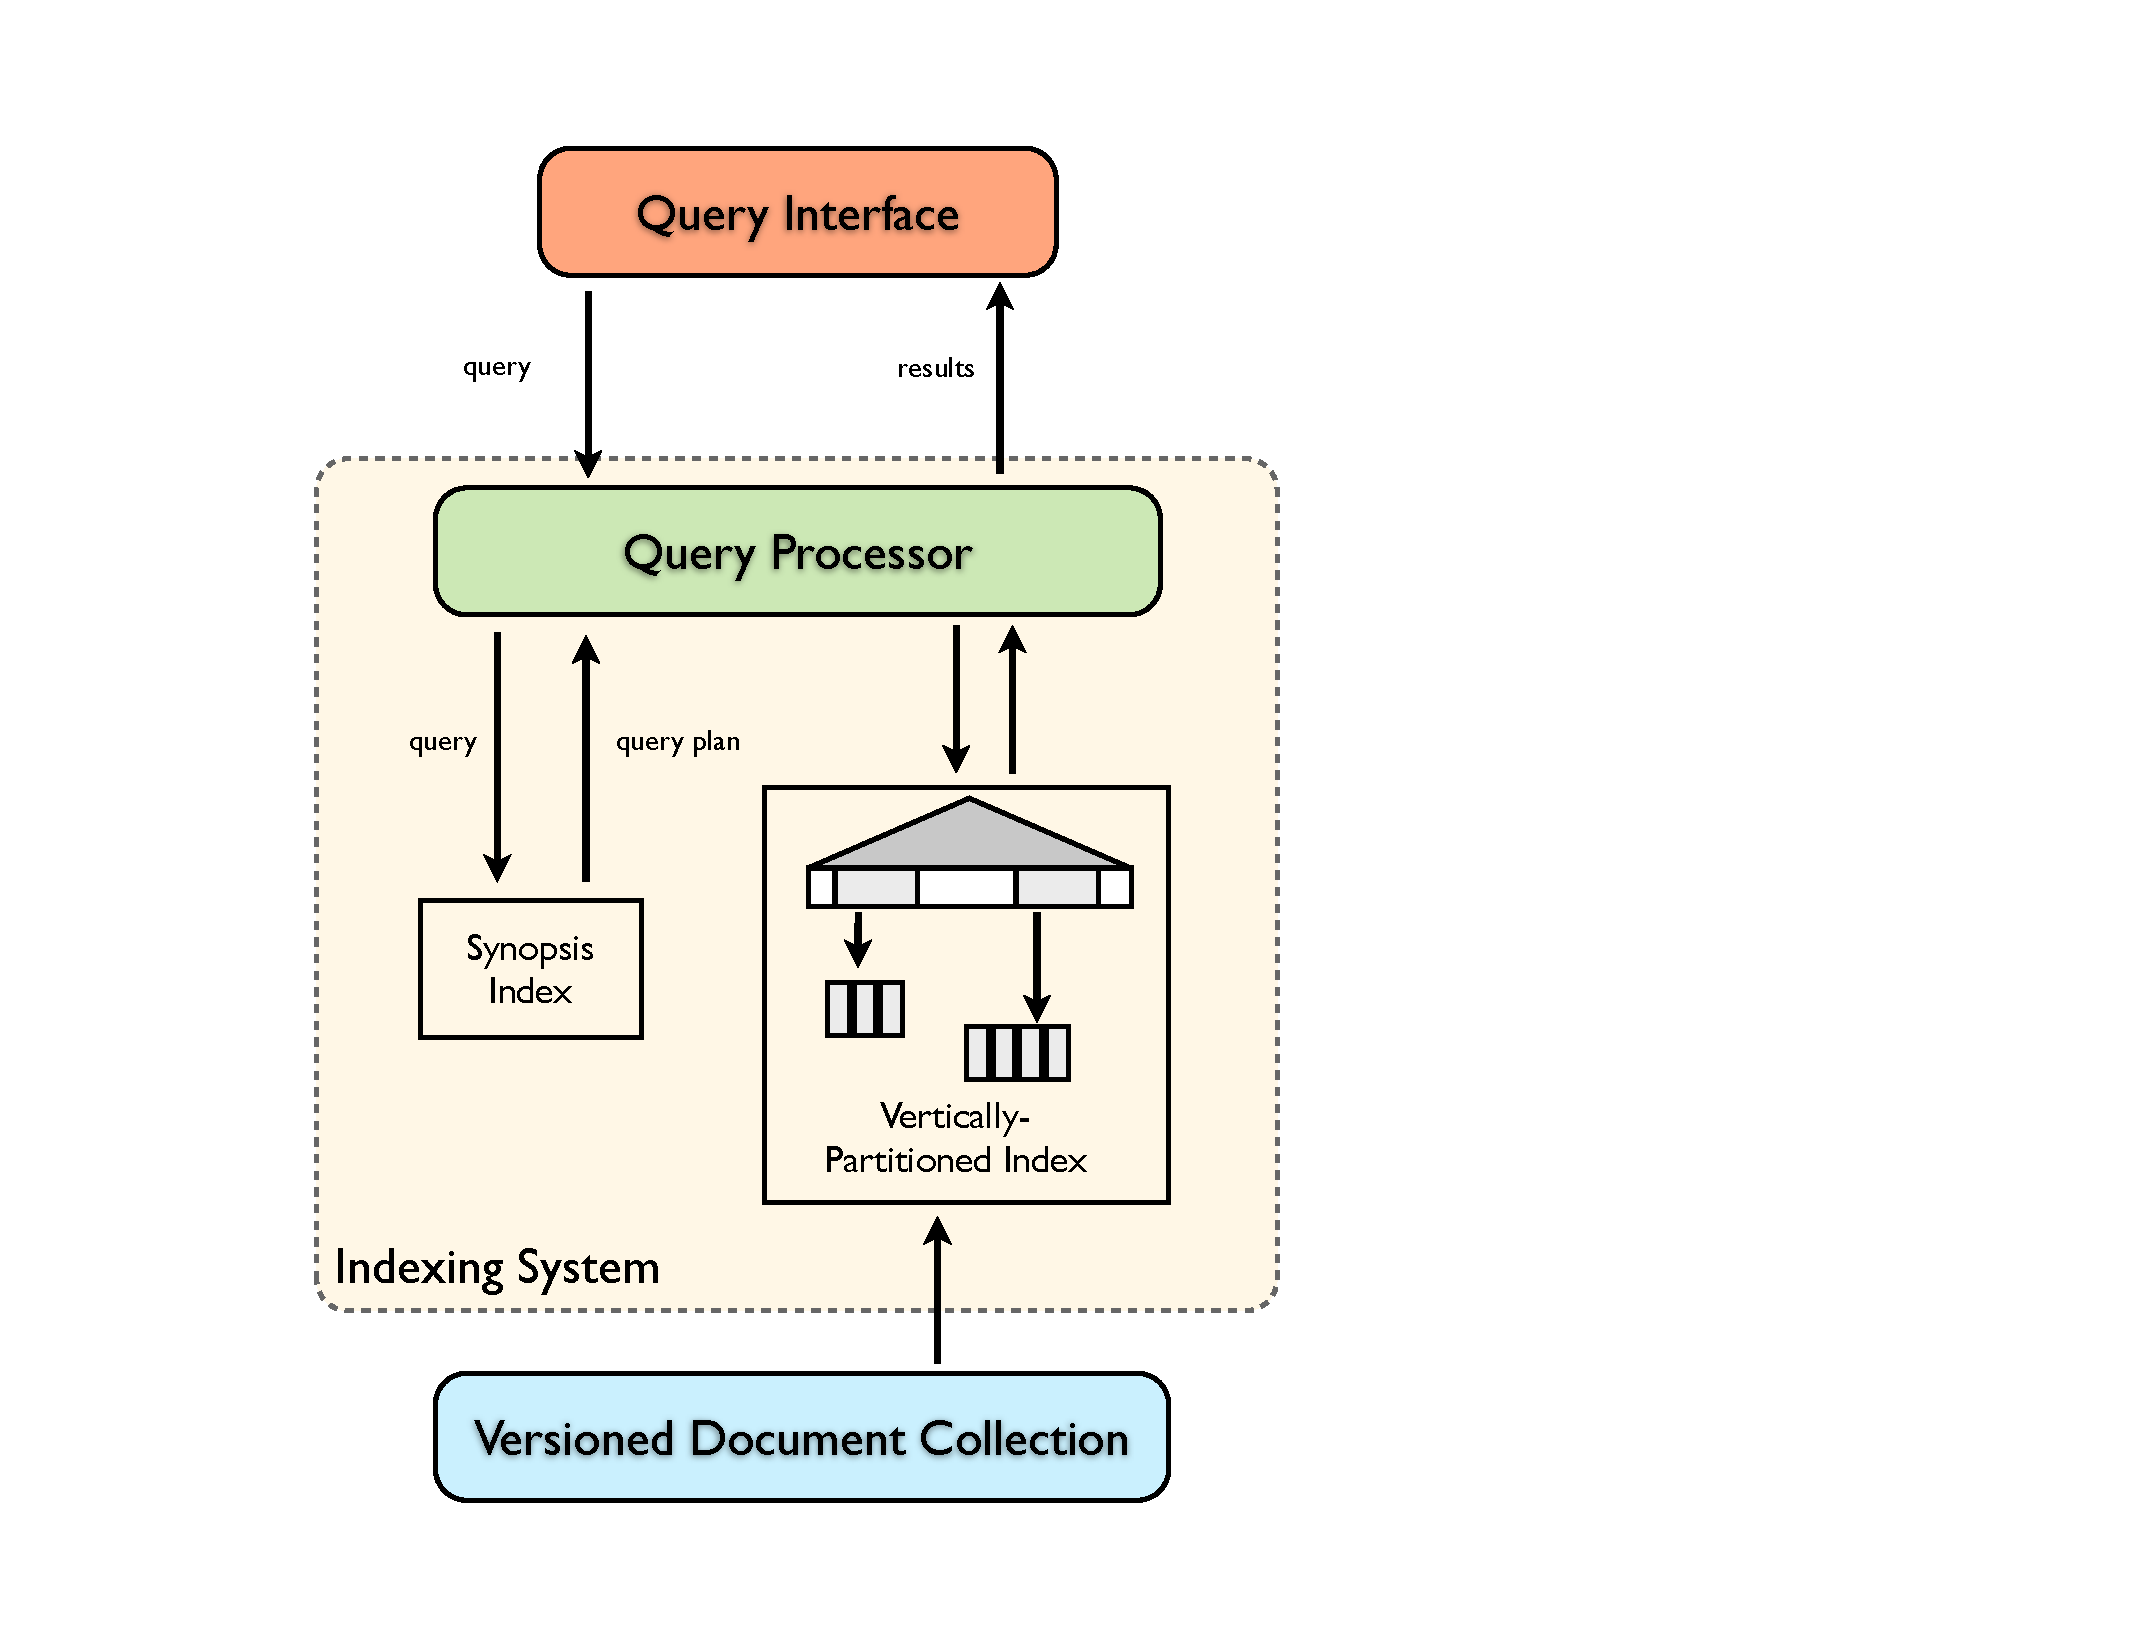
\includegraphics[width=0.6\columnwidth]{resources/selection-sysarch.pdf}
  \caption{System architecture} 
    \label{fig:selection_sysarch}
\end{figure}

Figure~\ref{fig:selection_sysarch} shows a hihg-level overview of the indexing system where our selection methods can be employed. The indexing system consists of \emph{vertically-partitioned index} and the \emph{synopsis index}.

\begin{itemize}

\item{\textbf{Vertically-partitioned index :}} The entire document collection is indexed employing the partitioning schemes described in~\cite{kberberi:sigir2007}. 

\item{\textbf{Synopsis Index :}} During index building we materialize a KMV synopsis for every partition into a \emph{synopsis index}. When a query is issued, synopses (i.e., multiple synopsis) corresponding to the affected partitions are retrieved. In the partition selection algorithm that follows, \textsc{GreedySelect} for single and multi-terms, cardinality estimates are determined for benefit values $B_i$ and $B_\mathbf{x}$.

\end{itemize}

The query interface can be a user of a system which generates time-travel queries. During processing queries, query optimization is performed on the synopsis index by invoking the selection algorithms and a plan is generated. Based on the query plan, accesses are scheduled on the vertically-partitioned index and the results are reported. Because of the anytime nature of the selection algorithm, the user can terminate the search, when satisfied, giving her the maximum recall computed thus far.

\section{Practical Issues}
While the previous two sections presented the theoretical
underpinnings for the partition-selection problem, in this section, we discuss a few
issues relevant to their implementation that we faced in practice and
present our solutions.

% \subsection{Using KMV synopsis for partition selection}
% As we discussed earlier, we use KMV synopsis for estimating the cardinality of the set-based operations in the proposed selection algorithms. During index building we materialize a KMV synopsis for every partition into a \emph{synopsis index}. When a query is issued, synopses (i.e., multiple synopsis) corresponding to the affected partitions are retrieved. In the partition selection algorithm that follows, \textsc{GreedySelect} for single and multi-terms, cardinality estimates are determined for benefit values $B_i$ and $B_\mathbf{x}$.

\subsection{Dealing with Partition and Query Boundary Alignment}
In our descriptions of the algorithms, we assumed that if a partition
overlaps with the query time-interval, then its contribution to the final
answer set is from \emph{all the postings} in the partition. In other
words, we ignored the fact that even within a partition, possibly a
large number of postings may not satisfy the temporal predicate if
the temporal boundaries of the partition are not completely contained
within the range specified by the temporal predicate. Note that this
affects the estimates of the \emph{benefit} values of the partitions
in the boundaries of the query time -- thus the benefits of at most 2 partitions per term are in error.

This error can be significantly improved if we adjust the value of
benefit of a partition to account for incomplete overlap along the
time axis. A straightforward approach for this, which we employ in our
implementation, is to \emph{scale} the benefits by the fraction of
temporal overlap between the query and the partition. In practice,
we observed that this simple scaling (which is similar to making an uniformity assumption during cardinality estimates) works very well.


\subsection{I/O Budget Underflow}
Another issue that comes up when we are using only \emph{estimates} of
benefit provided by partition(s) towards the final answer set is that
during partition selection, we may encounter a situation where
\emph{none of the partitions} show any non-zero benefit, although in
reality they may contain some results. When faced with such a
situation, the partition selection algorithms described in
Sections~\ref{sec:psmtq} and~\ref{sec:singleterm-selection} simply terminate -- even if the specified
I/O budget allows for more partitions to be read. 

To avoid this undesirable behaviour, the partition-selection algorithm
can be modified to ignore the estimates of benefits when \emph{all}
the unselected partitions have zero estimated benefits. At this stage,
partitions are selected in \emph{decreasing} order of their size as
long as the I/O budget is not violated.

\section{Experimental Evaluation}
\label{chap:selection:sec:evaluation}


\subsection{Evaluation Framework}
\label{sec:evaluation_framework}

In this section, we present and discuss the results of a detailed
experimental evaluation of our algorithms in terms of their
effectiveness in achieving high relative recall with a specified budget of index accesses.

\subsection {Setup}
All our algorithms, including the underlying time-travel inverted
index framework, were implemented using Java 1.6.
All experiments were conducted on Dell PowerEdge M610 servers
with 2 Intel Xeon E5530 CPUs, 48 GB of main memory, a large
iSCSI-attached disk array, and Debian GNU/Linux (SMP Kernel
2.6.29.3.1) as operating system. Experiments were conducted using
the Java Hotspot 64-Bit Server VM (build 11.2-b01).

\subsection{Datasets Used}
For our experiments we used three different datasets, all derived from
real-world data sources.

\begin{description}
\item[WIKI]
%\noindent\textbf{WIKI.}
{ The \emph{English Wikipedia revision history}
    \cite{wiki}, whose uncompressed raw data amounts to 0.7~TBytes,
    contains the full editing history of the English Wikipedia from
    January~2001 to December~2005. We indexed all versions of
    encyclopedia articles excluding versions that were marked as the
    result of a minor edit (e.g., the correction of spelling errors
    etc.). This yielded a total of 1,517,524 documents with 15,079,829
    versions having a mean ($\mu$) of 9.94 versions per document at
    standard deviation ($\sigma$) of 46.08.}
    
\item[UKGOV]
%\noindent\textbf{UKGOV.}
{ This is a subset of the European
    Archive~\cite{ea}, containing weekly crawls of eleven
    governmental websites from the U.K. We filtered out documents not
    belonging to MIME-types \texttt{text/plain} and
    \texttt{text/html} to obtain a dataset that totals 0.4~TBytes.
    This dataset includes 685,678 documents with 17,297,548 versions
    ($\mu = $ 25.23 and $\sigma = $ 28.38).}

\item[NYT]
%\noindent\textbf{NYT.}
{ The \emph{New York Times
      Annotated corpus}~\cite{NYT} comprises more than
    1.8 million articles from the New York Times published between
    1987 and 2007. Every article has an associated time-stamp which
    was taken as the begin time for that article. The end time for
    each article was chosen to be 90 days after the begin time, giving
    every document a validity time of 90 days. This is done to reflect
    the real world setting where the news articles are publicly
    available only for a limited period from their publication. }
    
\end{description}
Note that each of these datasets represents a realistic class of time-varying text collection typically used in temporal text
analytics. Specifically, WIKI corresponds to an explicitly version
controlled text collection, UKGOV is an archive of the evolving Web,
and NYT is an instance of archive of continually generated newspaper
content. For the ease of experimentation, we rounded the
time-stamps of versions to the nearest day for all datasets.

\subsection{Query Workload}

We compiled three dataset-specific query workloads by extracting
frequent queries from the AOL query logs, which were temporarily made
available during 2006. For the WIKI dataset we extracted 300 most
frequent queries which had a result click on the domain
\texttt{en.wikipedia.org} and similarly for NYT and UKGOV we compiled
300 queries which had a result hit on \texttt{nytimes.com} and
50 queries which had result hit on \texttt{.gov.uk} domains (cf. Appendix).  Using these keyword queries, we generated a
time-travel query workload with 3 instances each for the following 2
different temporal predicate granularities: 30 days and 1 year. 

%Thus, for each dataset, a query workload consisting of 15,000 ($=300 \textrm{ keyword queries} \times 5 \textrm{ temporal   granularities} \times 10 \textrm{ instances}$) was prepared.


\subsection{Index Management}

\begin{table*}[!ht]
\centering
\begin{tabular}{@{}llrcrcr@{}}\toprule
 \multicolumn{2}{l}{\textbf{Index}}& \multicolumn{1}{c}{\textbf{UKGOV}} & \phantom{ab} & \multicolumn{1}{c}{\textbf{NYT}}& \phantom{ab} & \multicolumn{1}{c}{\textbf{WIKI}}\\ 
 \midrule
    Fixed-7 && 11GB && 13GB && 13GB \\
    Synopsis Index - 5\% sample && 146MB && 134MB && 146MB \\
    Synopsis Index - 10\% sample && 291MB && 258MB && 290MB \\
\midrule
    Fixed-30 && 4.4GB && 3.5GB && 6.3GB \\
    Synopsis Index - 5\% sample && 61MB && 39MB && 75MB \\
    Synopsis Index - 10\% sample && 122MB && 74MB && 149MB \\
 
 \bottomrule
\end{tabular}
\caption{Synopsis index}
  \label{tab:syndex}
\end{table*}

Since our selection techniques operate on temporally-partitioned posting lists, we chose the following partitioning schemes :

\begin{itemize}
  \item \textbf{Fixed-time partitioning} A simple partitioning scheme in which a partition boundary is placed after a fixed time window. We present results for two time window sizes: (i) 1 week (referred to as
{\bf Fixed-7} partitioning), and (ii) 1 month (referred to as {\bf
  Fixed-30} partitioning). Unless otherwise mentioned, all the results
presented in this chapter are from {\bf Fixed-7} partitioning.

\item {\bf Vertical Partitioning} These are index structures built using partitioning strategies discussed in~\cite{kberberi:sigir2007}). More specifically, we build index structures using the \emph{space-bound approach} with the parameters $\kappa=1.5 , 3.0$ as two representatives of lower and higher degree of partitioning. These are represented as {\bf VERT-1.5} and {\bf VERT-3.0} respectively.

\end{itemize}

Each of the above time-travel inverted indexes is stored on disk using flat files containing both the lexicon as well as posting lists. At run time, the lexicon is read completely into memory, and for a given query the
appropriate partition is retrieved from the index flat file on
disk. These posting lists are stored using variable-byte compression. 

\paragraph{Synopsis structures} The estimates from the KMV synopses~\cite{kmv:sigmod} that we
chose to implement are naturally dependent on their size in relation
to the raw data size. We experimented with two sizes of synopses: 5\%
and 10\% of the partition size (with minimum size set to 100). Unless
otherwise mentioned, we report results for 10\% size of the KMV synopsis. A synopsis index was generated during index construction time and stored as flat files on disk. Instead of storing the list of hashed double values of the KMV synopsis, the corresponding document identifiers (32-bit integers) were stored for better compression (Table~\ref{tab:syndex}). The document identifiers were translated to their respective doubles during query time for the necessary KMV intersection estimation. An additional entry in the lexicon was stored the offset in the synopsis index file corresponding to the synopsis for each partition.

% The
% synopses structures, one for each partition, was computed using KMV synopsis and were maintained in a separate flat file in a similar way as the inverted index. 
Finally, we employed a practically infeasible {\bf oracle} for partition
selection, which computes the \emph{accurate values} of set operations
(intersection and union) between partitions. Oracle computes these
values by simply evaluating the query completely, without any
partition selection, and then uses them in partition selection to overcome the errors due to estimates from the KMV synopses. 
In our experiments, we consider the oracle as a competitor, where  exact cardinalities are known, to compare against our synopsis-based-selection approaches. 

\subsection{Evaluation Methodology}

We evaluate the impact of partition selection by measuring the recall obtained at different values of the parameter $\beta$. In each experiment we measure the average recall value obtained per query, for a certain selection method, over increasing values of $\beta$ from 0 to 1 with a step size of 0.1. During averaging we exclude the measurements for two types of queries. First, we exclude queries with term/s not in the lexicon as they contribute to false-positives for partition selection. Since we employ conjunctive query semantics we need to select at least one partition per-term. Thus, secondly we also ignore queries which result in exactly one affected partition for each term.

% Further, we treat queries which have the answer set size of
% $0$ (i.e., there are no results which satisfy both keyword and
% temporal predicates) as contributing a perfect recall, as our
% estimations can accurately determine these. 
To compare the I/O performance of different techniques, we measure the
number of postings read after applying partition selection --
denoted as {\bf RWS}, and the number of postings read without
applying partition selection -- denoted as {\bf RWOS}. The ratio
$\frac{RWS}{RWOS}$, called \emph{Ratio-of-index read}, is denoted as
{\bf RIR}. The ratio-of-index read captures the amount of index accessed relative to the overall index-access cost for processing the entire query. We also measure the wall-clock times during query processing, reported in milliseconds.

%\subsection{Experimental Results}

%\begin{figure*}[ht!]
\begin{figure*}
  \centering
  \subfigure[Wikipedia]{\label{fig:vary_time_wiki_pse_fixed_7d}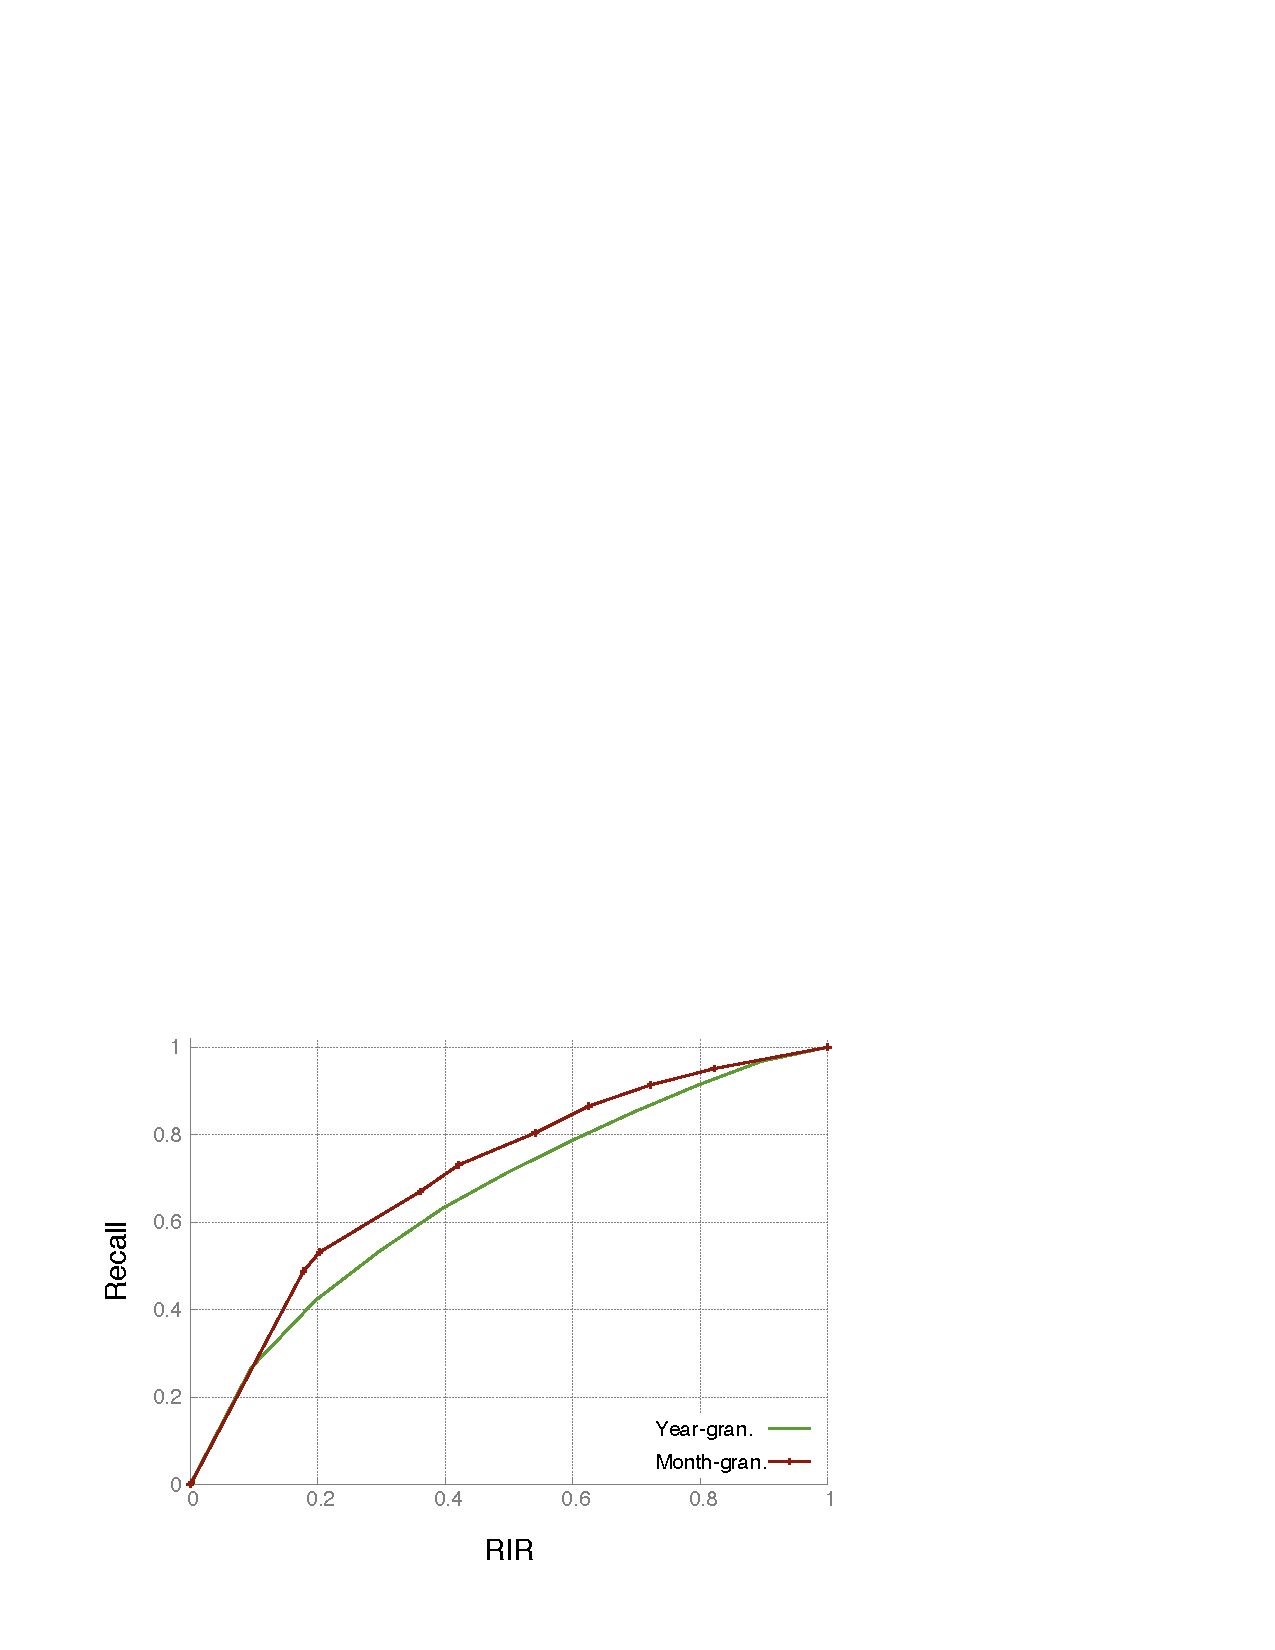
\includegraphics[width=0.60\textwidth]{plots/selection/cc_results/round2/pdf/wiki-time-interval-granularity-pse-7days.pdf}}
  \subfigure[UKGOV]{\label{fig:vary_time_ukgov_pse_fixed_7d}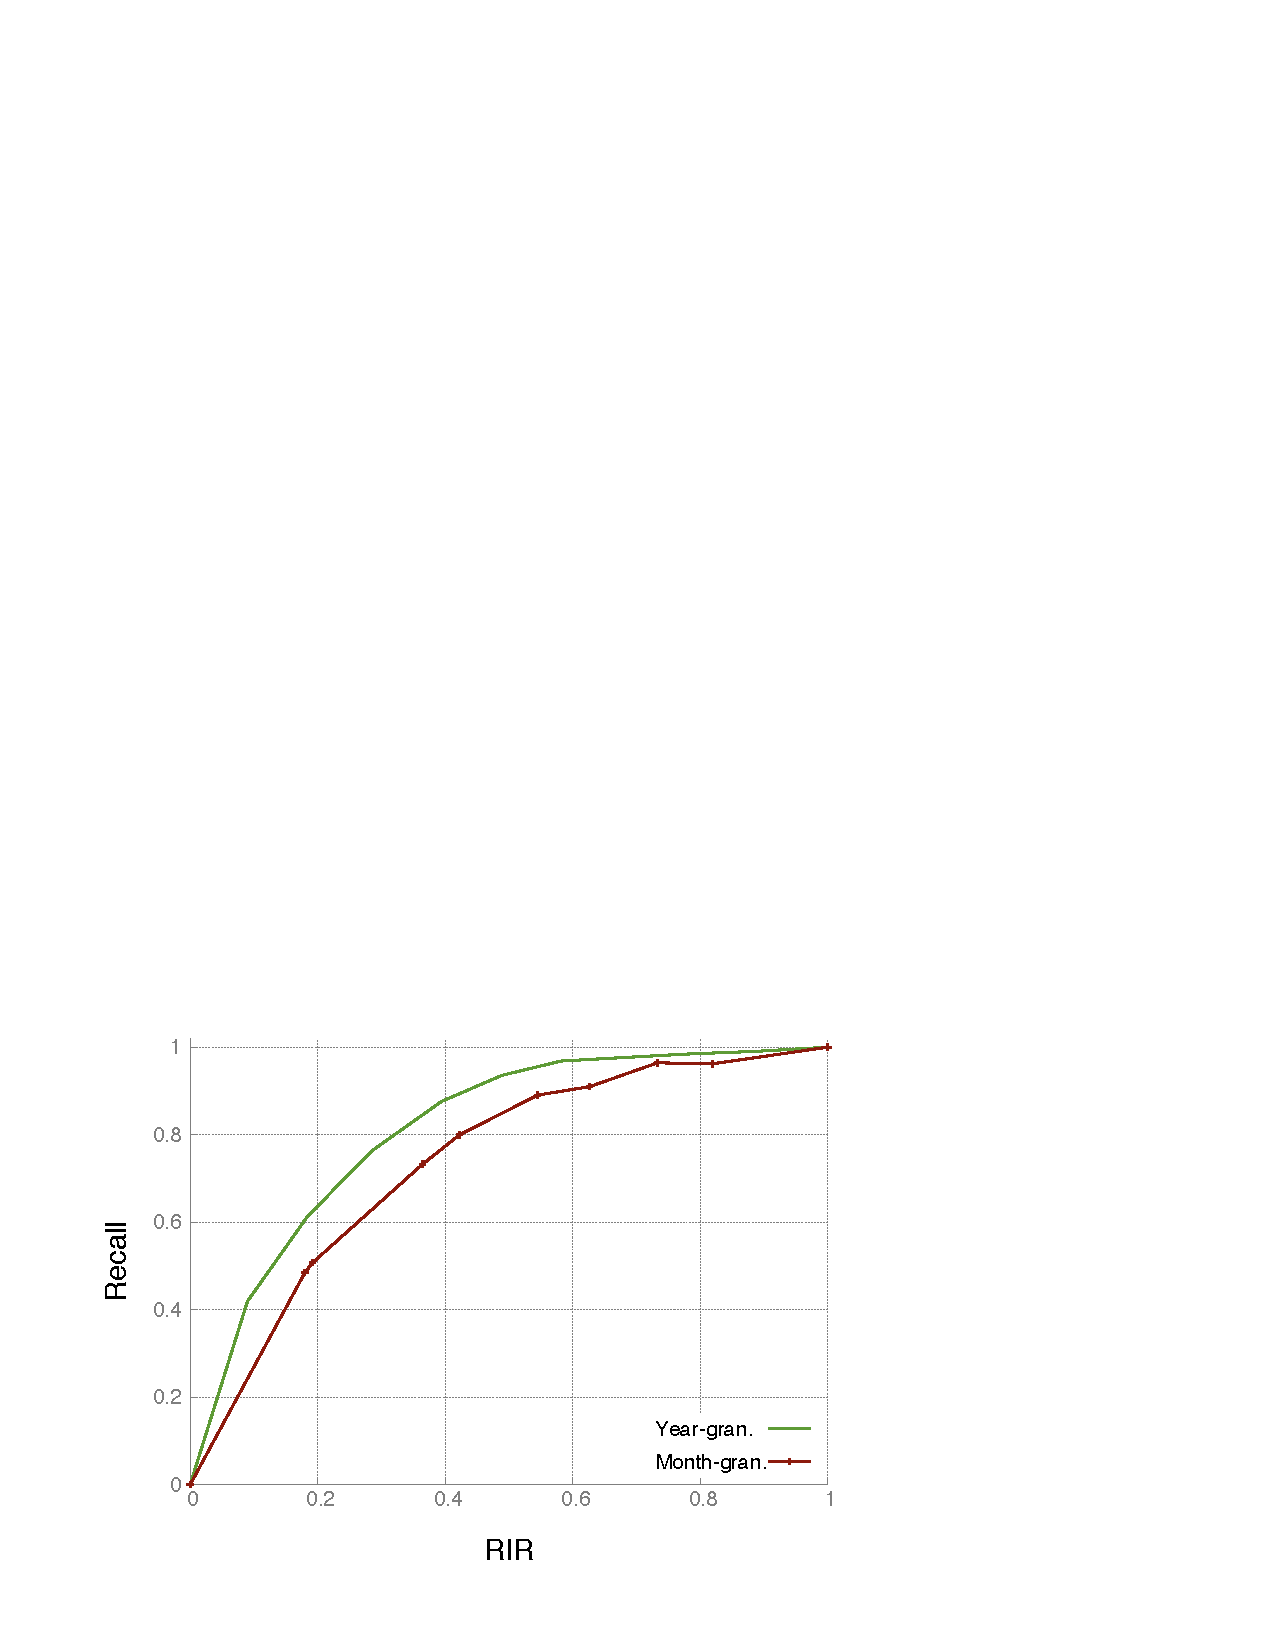
\includegraphics[width=0.60\textwidth]{plots/selection/cc_results/round2/pdf/ukgov-time-interval-granularity-pse-7days.pdf}}
  \subfigure[New York
  Times]{\label{fig:vary_time_nyt_pse_fixed_7d}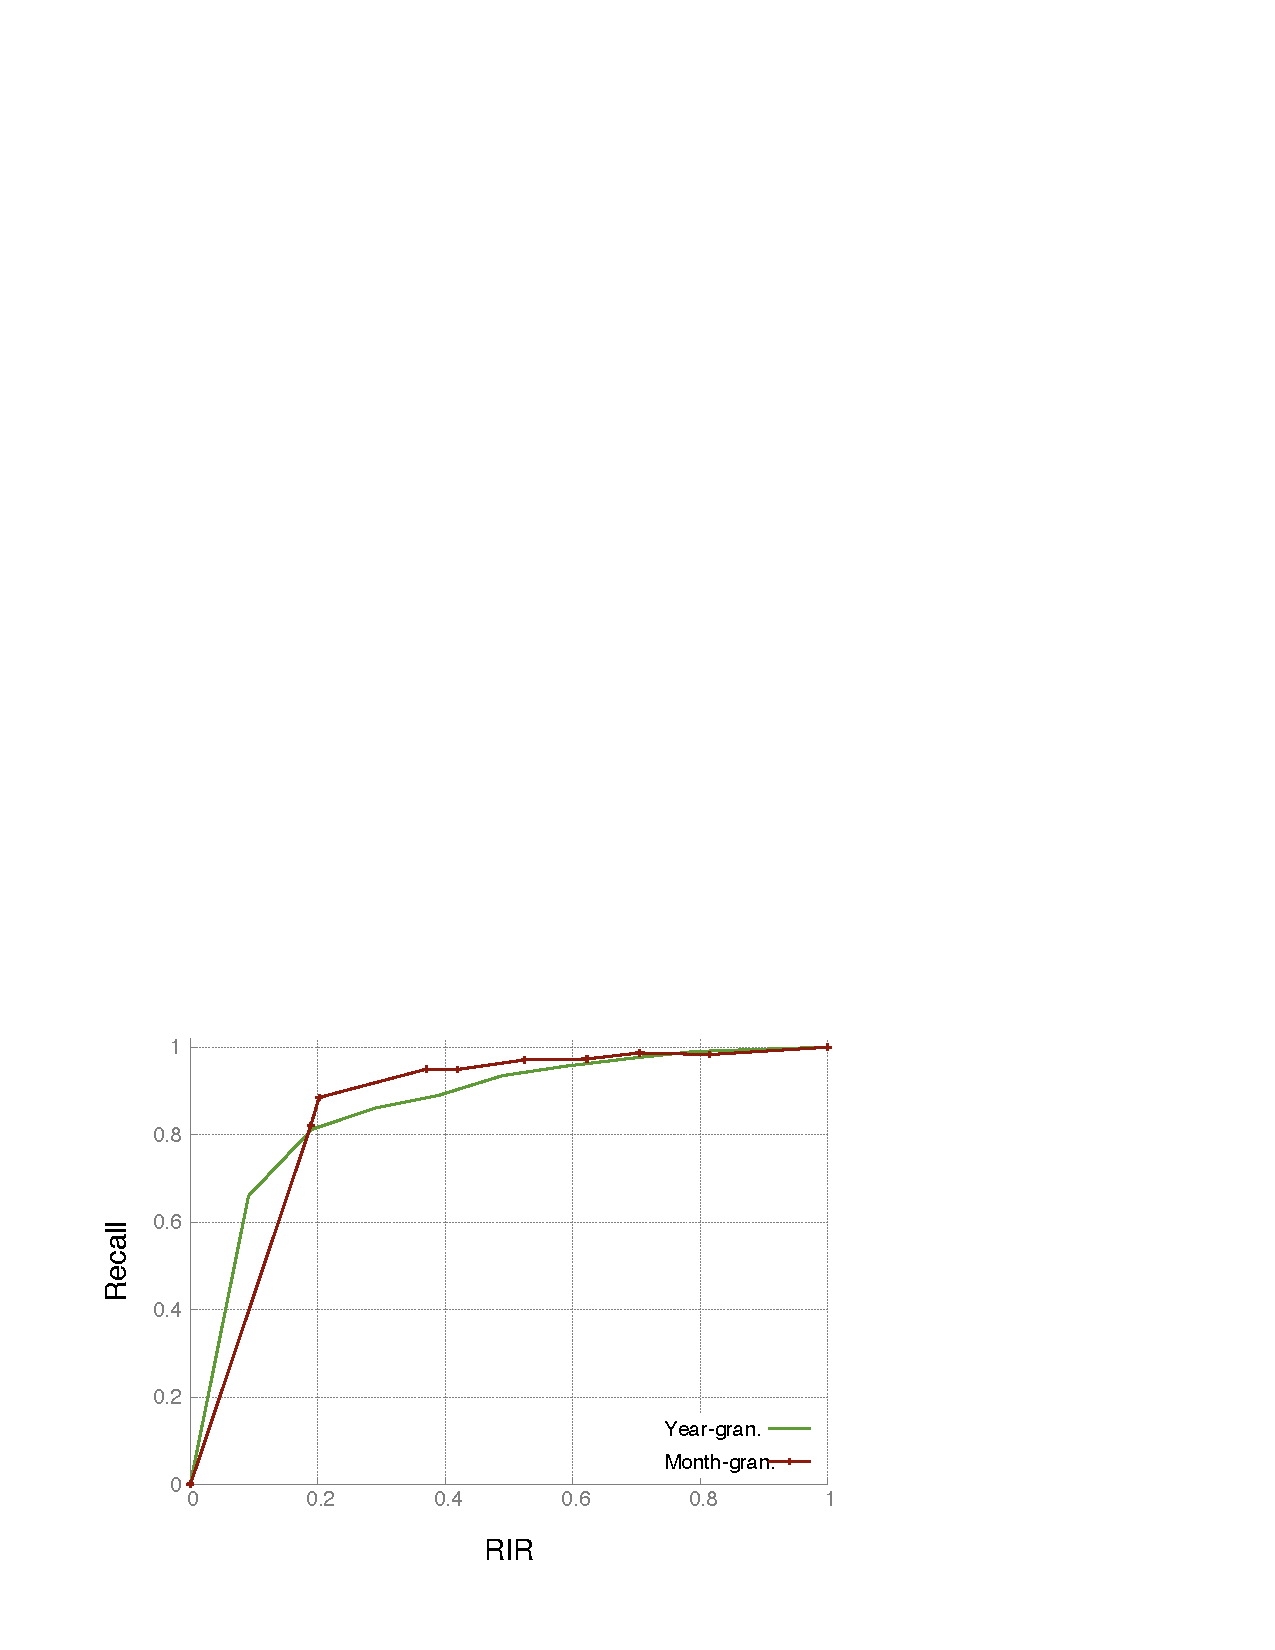
\includegraphics[width=0.60\textwidth]{plots/selection/cc_results/round2/pdf/nyt-time-interval-granularity-pse.pdf}}
  
  \caption{Performance of size-based partition selection on Fixed-7 index}
  \label{fig:pse_query_times}
\end{figure*}

%\begin{figure*}[ht!]
\begin{figure*}
  \centering
  \subfigure[Wikipedia]{\label{fig:vary_time_wiki_psp_fixed_7d}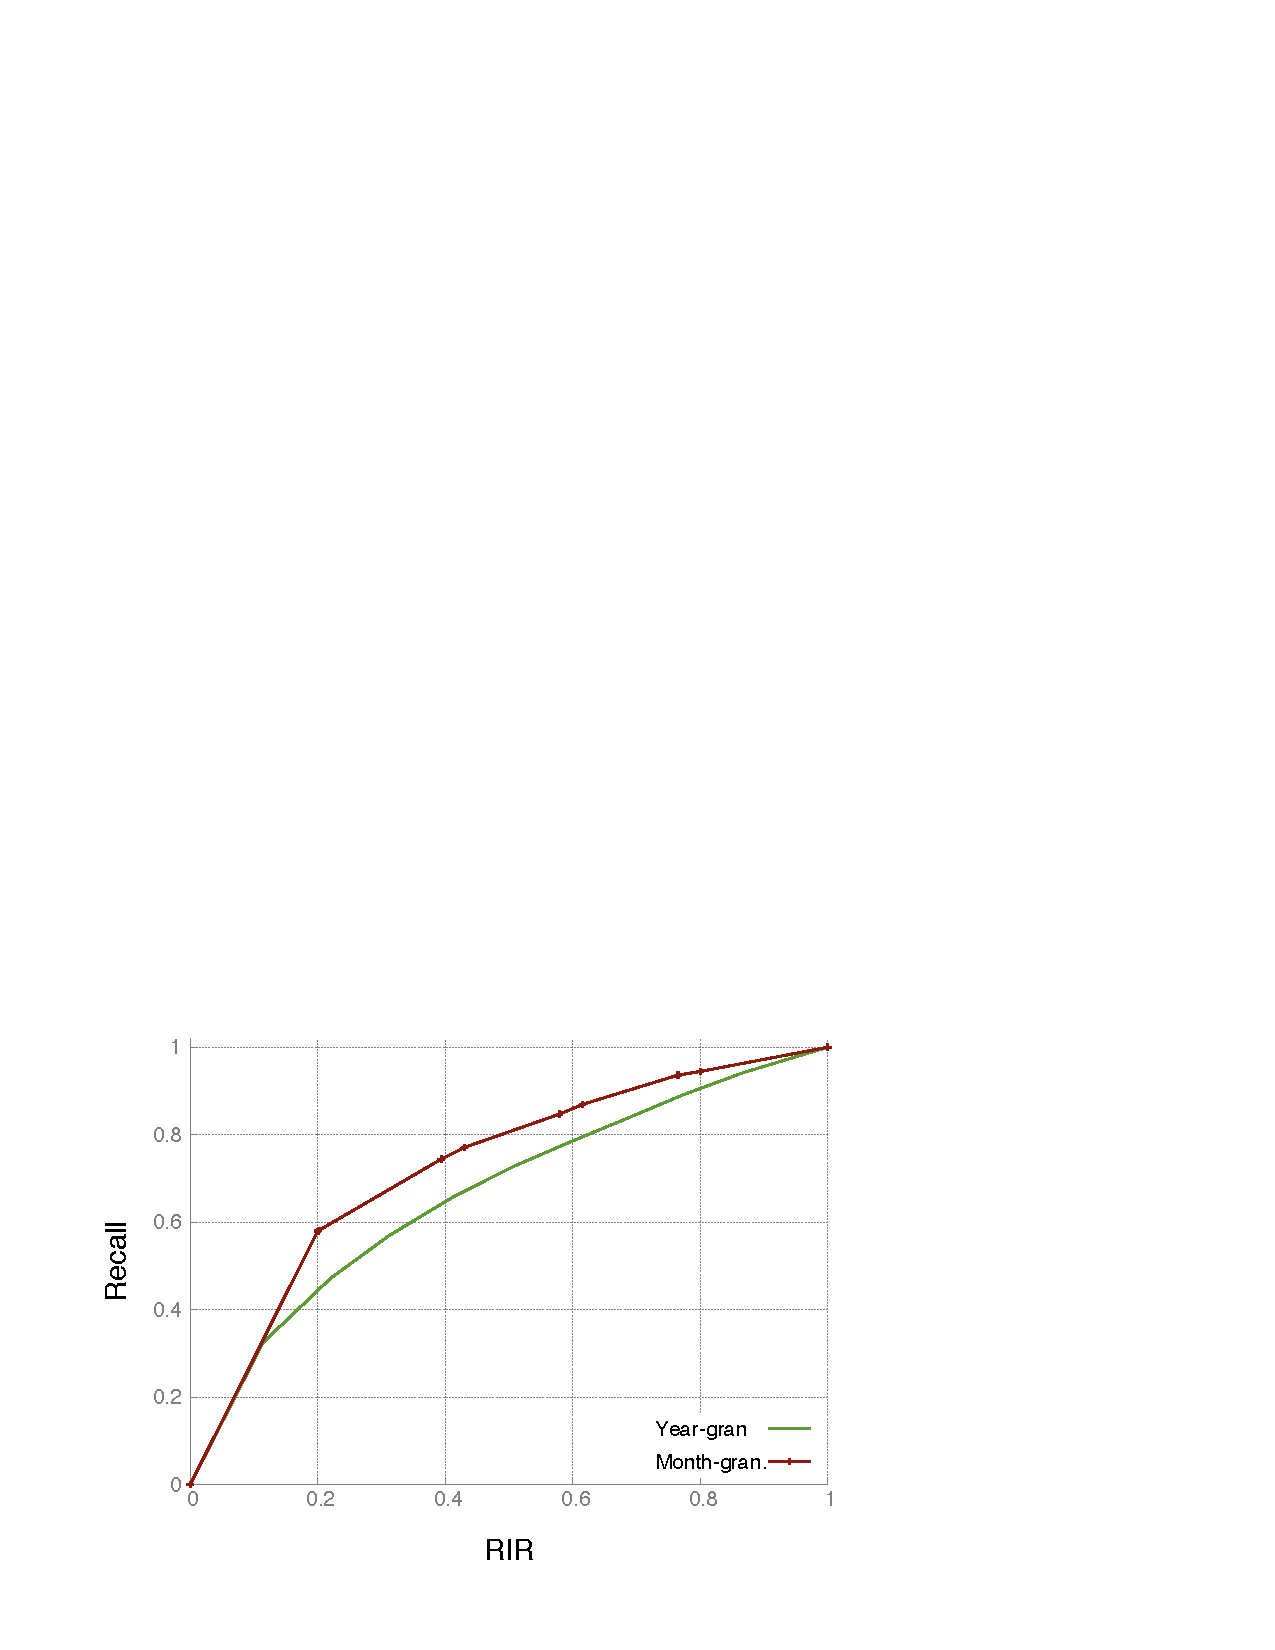
\includegraphics[width=0.60\textwidth]{plots/selection/cc_results/round2/pdf/wiki-time-interval-granularity-psp-7days.pdf}}
  \subfigure[UKGOV]{\label{fig:vary_time_ukgov_psp_fixed_7d}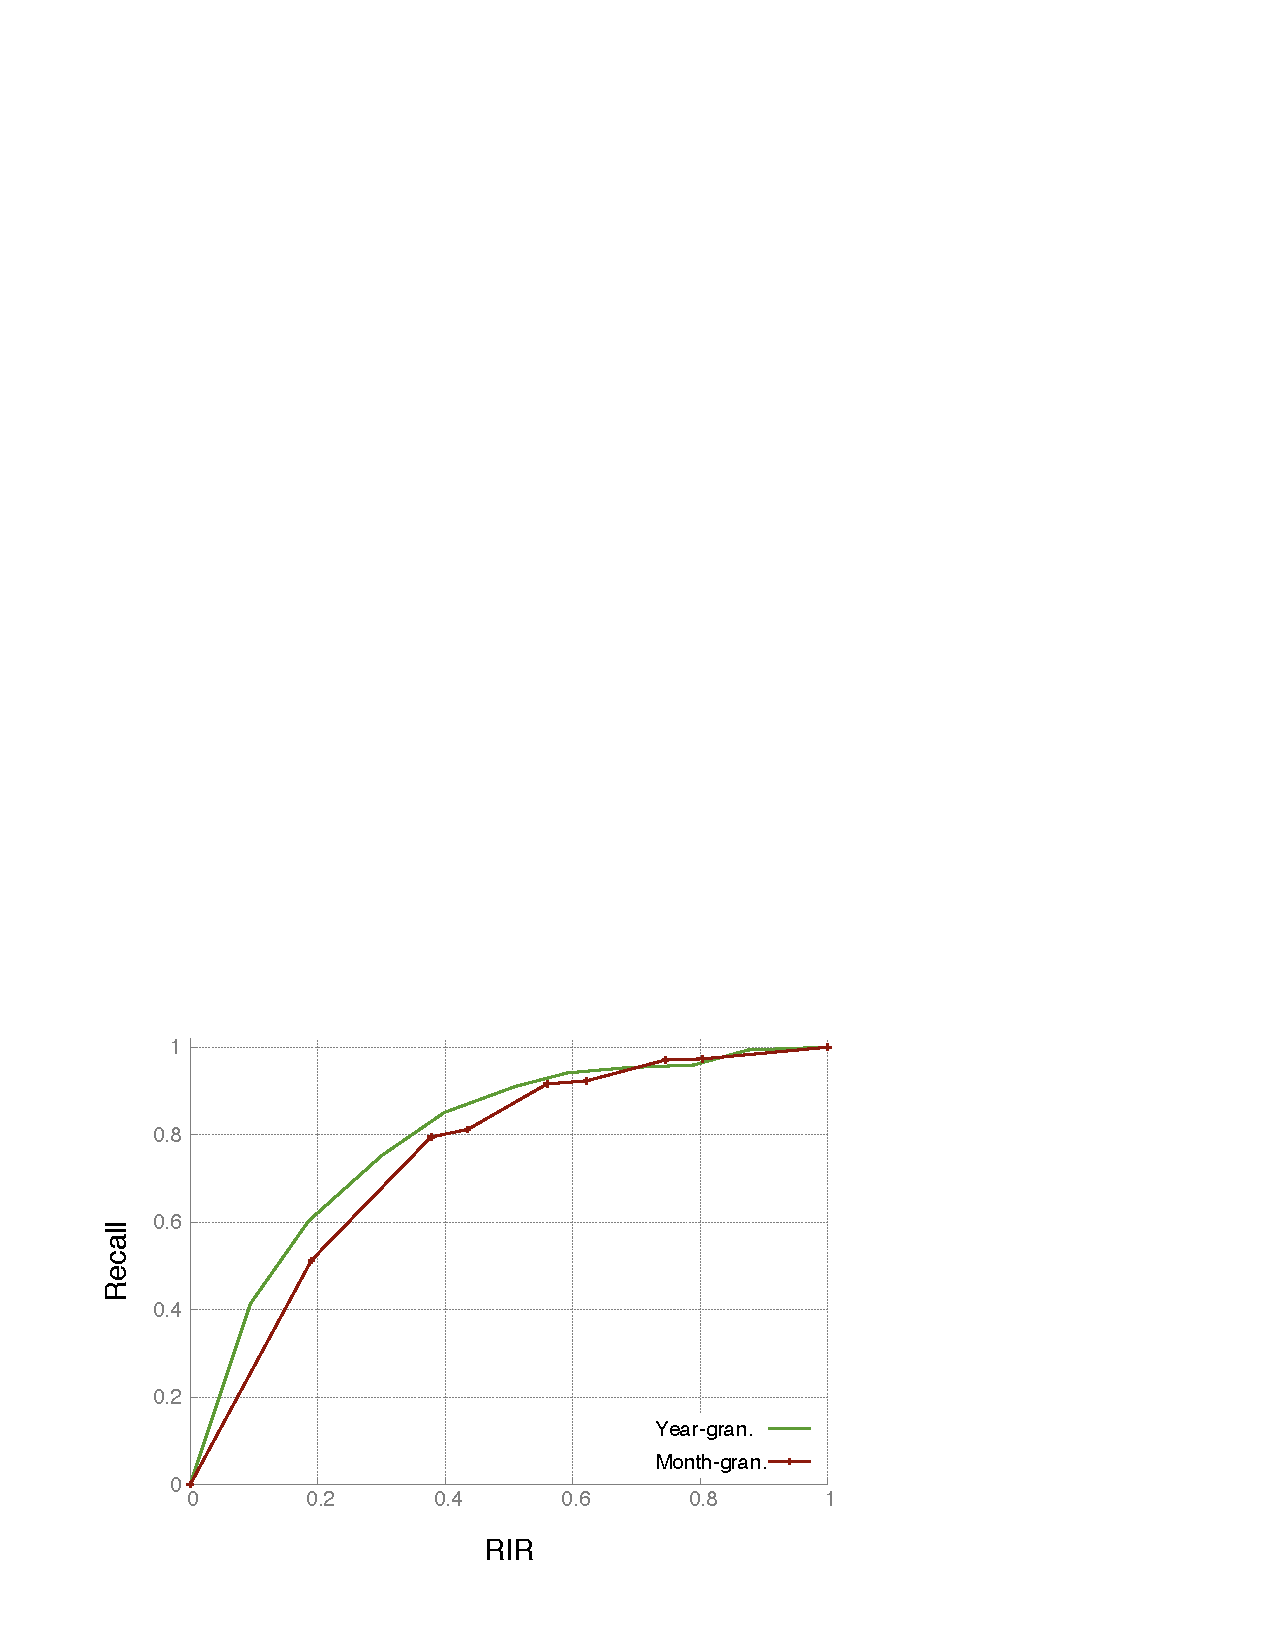
\includegraphics[width=0.60\textwidth]{plots/selection/cc_results/round2/pdf/ukgov-time-interval-granularity-psp-7days.pdf}}
  \subfigure[New York
  Times]{\label{fig:vary_time_nyt_psp_fixed_7d}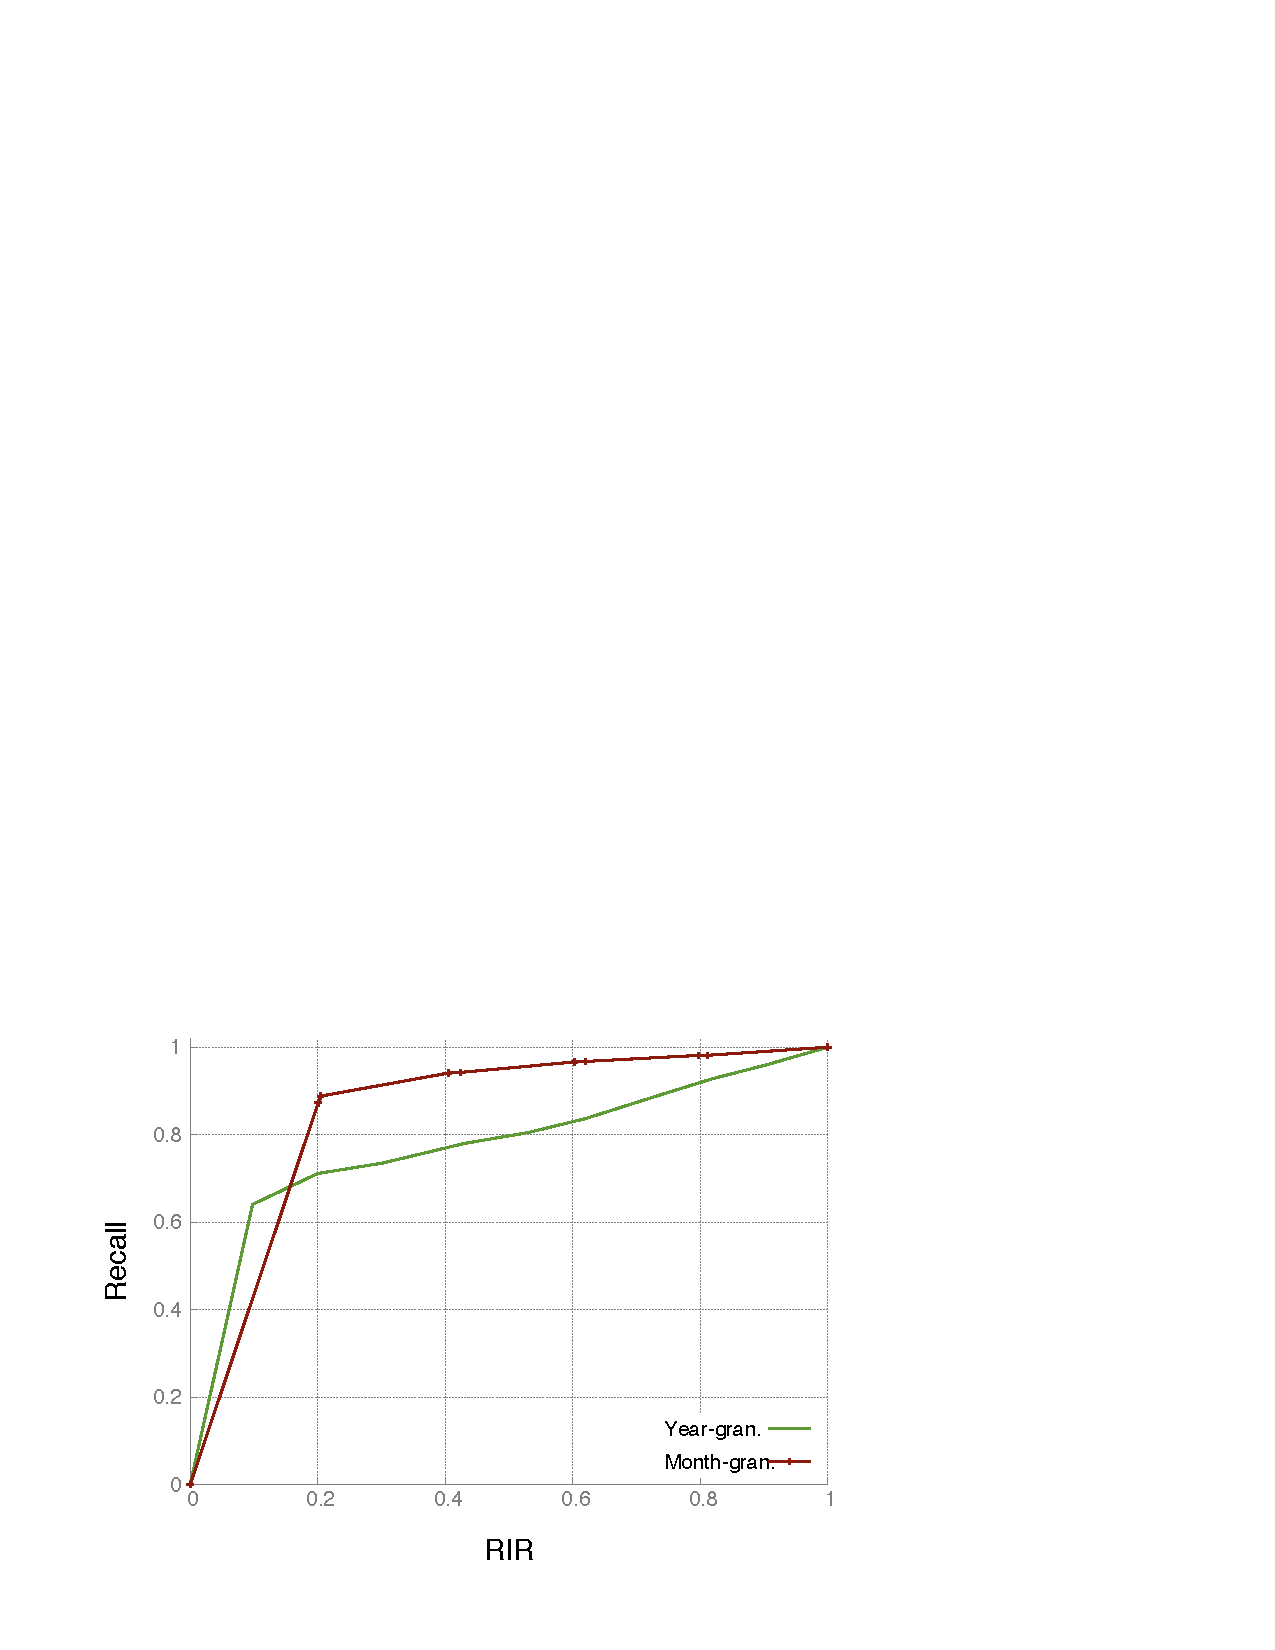
\includegraphics[width=0.60\textwidth]{plots/selection/cc_results/round2/pdf/nyt-time-interval-granularity-psp-7days.pdf}}
  	
  \caption{Performance of equi-cost partition selection on Fixed-7 index}
  \label{fig:psp_query_times}
\end{figure*}

%\begin{figure*}[ht!]
\begin{figure*}
  \centering
  \subfigure[Wikipedia]{\label{fig:vary_time_wiki_pse_sb2.5}\includegraphics[width=0.6\textwidth]{plots/selection/cc_results/round2/pdf/wiki-time-interval-granularity-psp-sb.pdf}}
  \subfigure[UKGOV]{\label{fig:vary_time_ukgov_pse_sb2.5}\includegraphics[width=0.6\textwidth]{plots/selection/cc_results/round2/pdf/ukgov-time-interval-granularity-psp-sb.pdf}}
  \subfigure[New York Times]{\label{fig:vary_time_nyt_pse_sb2.5}\includegraphics[width=0.6\textwidth]{plots/selection/cc_results/round2/pdf/nyt-time-interval-granularity-psp-sb.pdf}}
  
  \caption{Performance of size-based partition selection on VERT-3.0 index}
  \label{fig:pse_query_times_sb}
\end{figure*}

\subsection{Performance of Partition Selection}
\label{sec:exp_ps}

% In the first set of experiments, we demonstrate the impact of using
% partition selection in identifying the set of partitions that maximize
% the final result recall. As described earlier, the I/O budget can be specified in two forms -- based on size of partitions, or based on the number of
% partitions. For both the budget formulations, we ran the full query
% workload for each of the datasets, and present aggregated results
% individually for every query time-window. The results are plotted in
% Figure~\ref{fig:pse_query_times} for size-based selection, and in
% Figure~\ref{fig:psp_query_times} for equi-cost partition selection
% approaches.

In the first set of experiments, we examine the impact of both the selection methods described in this chapter - size-based selection and equi-cost selection. To this end, we execute the different query granularities on the \textbf{Fixed-7} index for the given datasets, and measure the recall values at various stages of query execution. The cost incurred at a given stage of query execution is measured, as introduced above, by RIR. The results presenting the recall levels achieved at different RIR values are shown in Figure~\ref{fig:pse_query_times} (size-based selection) and Figure~\ref{fig:psp_query_times} (equi-cost partition selection).

We observe that both selection algorithms achieve perfect recall already when accessing about 50\% of the index. Since both the algorithms are incremental in nature, recall always increases with an increase in allowable I/O budget $\beta$. Both the selection methods are able to achieve a recall of 80\% by accessing less than 30\% of the affected postings for NYT. In UKGOV, a 80\% recall is achieved by accessing 40\% of the index. In WIKI, the results are not as temporally clustered as in NYT and UKGOV but we still reach 80\% of recall by accessing around 60\% of the affected postings. 

Next, we observe that, with the exception of UKGOV, the partition-selection methods respond better to month-granularity queries than the year-granularity queries. Month-granularity queries have fewer affected partitions than year-granularity queries. This suggests that there is (i) a high degree of temporal clustering of results and (ii) high replication of postings, which the selection methods exploit. Selecting the partitions with a high concentration of results gives the observed boost to the recall levels. The subsequent choice of partitions understandably adds lower improvement than the initial choices exhibiting the property of diminishing returns. When we conducted the same experiment on the vertically-partitioned index VERT-3.0, we did not observe gains as significant as in \textbf{Fixed-7}. This is because the replication of the postings is controlled and bounded. 

The final observation which we make is that both the selection methods perform almost at par. There is no considerable difference in performance and the choices of partitions selected, in our experiments, is almost the same. This prompts the use equi-cost partition selection which is easier to implement and has a proven approximation guarantee. Thus from now on, the charts and tables contain results which employed equi-cost partition selection.

\begin{table*}\footnotesize
\centering
  % \begin{tabular}{@{}llccccccrr@{}}
  \begin{tabular}{@{}llrrrrrrrr@{}}
  \toprule
  \multicolumn{2}{l}{} & \multicolumn{2}{c}{\textbf{Year Granularity}} & \phantom{ab} & \multicolumn{2}{c}{\textbf{Month  Granularity}}\\ 
  \cmidrule{3-4} \cmidrule{6-7}
  &\textsc{Bound} & Recall & Wall-clock times (ms) && Recall & Wall-clock times (ms)\\
   \midrule
\textbf{WIKI}\\
& 0.1 & 0.27 & 207.6 && 0.01 & 5.7\\
& 0.2 & 0.42 & 367.7 && 0.49 & 88.5\\
& 0.3 & 0.53 & 436.8 && 0.53 & 94.3\\
& 0.4 & 0.63 & 521.0 && 0.67 & 134.3\\
& 0.5 & 0.71 & 594.8 && 0.73 & 135.9\\
& 0.6 & 0.78 & 646.7 && 0.80 & 165.2\\
& 0.7 & 0.85 & 736.3 && 0.87 & 165.9\\
& 0.8 & 0.91 & 798.5 && 0.91 & 186.4\\
& 0.9 & 0.97 & 877.4 && 0.95 & 192.0\\
\textsc{Noselection} & 1 & 1.00 & 1,020.8 && 1.00 & 212.0\\
\textsc{Nopartition} & 1 & 1.00 & 3,217.0 && 1.00 & 3,217.0\\
  \midrule
\textbf{UKGOV}\\
& 0.1 & 0.42 & 1,615.9 && 0.00 & 0.0\\
& 0.2 & 0.61 & 2,788.8 && 0.48 & 352.6\\
& 0.3 & 0.76 & 3,705.2 && 0.51 & 370.4\\
& 0.4 & 0.88 & 4,592.1 && 0.73 & 590.3\\
& 0.5 & 0.94 & 5,183.2 && 0.80 & 644.3\\
& 0.6 & 0.97 & 5,772.6 && 0.89 & 751.2\\
& 0.7 & 0.98 & 6,427.9 && 0.91 & 852.7\\
& 0.8 & 0.98 & 7,025.2 && 0.96 & 927.4\\
& 0.9 & 0.99 & 7,635.8 && 0.96 & 1,026.6\\
\textsc{Noselection}& 1 & 1.00 & 8,490.1 && 1.00 & 1,225.9\\
\textsc{Nopartition} & 1 & 1.00 & 12,598.0 && 1.00 & 12,598.0\\
\midrule
\textbf{NYT}\\
& 0.1 & 0.66 & 200.9 && 0.00 & 0.0\\
& 0.2 & 0.81 & 254.5 && 0.82 & 103.5\\
& 0.3 & 0.86 & 301.4 && 0.89 & 106.0\\
& 0.4 & 0.89 & 308.2 && 0.95 & 117.5\\
& 0.5 & 0.94 & 328.1 && 0.95 & 122.0\\
& 0.6 & 0.96 & 358.7 && 0.97 & 125.0\\
& 0.7 & 0.97 & 384.8 && 0.97 & 126.0\\
& 0.8 & 0.99 & 428.6 && 0.99 & 128.5\\
& 0.9 & 0.99 & 468.2 && 0.98 & 141.5\\
\textsc{Noselection}& 1 & 1.00 & 525.7 && 1.00 & 146.0\\
\textsc{Nopartition}& 1 & 1.00 & 1,014.0 && 1.00 & 1,014.0\\
   \bottomrule
  \end{tabular}
\caption{Wall-clock times for selection over Fixed-30}
\label{tab:selection_wct_fixed}
\end{table*}


\begin{table*}\footnotesize
  \centering
  % \begin{tabular}{@{}llccccccrr@{}}
  \begin{tabular}{@{}llrrrrrrrr@{}}
  \toprule
  \multicolumn{2}{l}{} & \multicolumn{2}{c}{\textbf{Year Granularity}} & \phantom{ab} & \multicolumn{2}{c}{\textbf{Month  Granularity}}\\ 
  \cmidrule{3-4} \cmidrule{6-7}
  &\textsc{Bound} & Recall & Wall-clock times (ms) && Recall & Wall-clock times (ms)\\
   \midrule
\textbf{WIKI}\\
& 0.1 & 0.28 & 105.8 && 0.26 & 12.8\\
& 0.2 & 0.43 & 154.4 && 0.42 & 33.4\\
& 0.3 & 0.55 & 212.2 && 0.55 & 44.0\\
& 0.4 & 0.65 & 268.1 && 0.62 & 55.5\\
& 0.5 & 0.73 & 320.5 && 0.70 & 64.6\\
& 0.6 & 0.81 & 375.6 && 0.77 & 75.6\\
& 0.7 & 0.87 & 429.4 && 0.84 & 87.4\\
& 0.8 & 0.92 & 477.6 && 0.89 & 97.2\\
& 0.9 & 0.96 & 539.0 && 0.93 & 104.3\\
\textsc{Noselection}& 1.0 & 1.00 & 596.4 && 1.00 & 129.0\\
\textsc{Nopartition} & 1.0 & 1.00 & 3,217 && 1.00 & 3,217.0\\
  \midrule
\textbf{UKGOV}\\

& 0.1 & 0.25 & 295.1 && 0.27 & 2.3\\
& 0.2 & 0.42 & 601.6 && 0.45 & 41.8\\
& 0.3 & 0.56 & 915.6 && 0.65 & 124.9\\
& 0.4 & 0.68 & 1260.7 && 0.73 & 172.3\\
& 0.5 & 0.78 & 1544.4 && 0.83 & 239.7\\
& 0.6 & 0.82 & 1803.1 && 0.87 & 271.1\\
& 0.7 & 0.87 & 2098.3 && 0.90 & 325.0\\
& 0.8 & 0.91 & 2265.2 && 0.94 & 358.7\\
& 0.9 & 0.94 & 2436.2 && 0.95 & 395.7\\
\textsc{Noselection}& 1 & 1.00 & 2720.2 && 1.00 & 572.7\\
\textsc{Nopartition} & 1 & 1.00 & 12,598 && 1.00 & 12,598.0\\

\midrule
\textbf{NYT}\\
& 0.1 & 0.28 & 26.7 && 0.00 & 0.0\\
& 0.2 & 0.50 & 53.0 && 0.18 & 1.0\\
& 0.3 & 0.62 & 50.87 && 0.32 & 3.0\\
& 0.4 & 0.76 & 54.9 && 0.47 & 11.8\\
& 0.5 & 0.83 & 60.6 && 0.61 & 21.4\\
& 0.6 & 0.87 & 65.3 && 0.71 & 19.9\\
& 0.7 & 0.92 & 72.4 && 0.81 & 24.1\\
& 0.8 & 0.95 & 81.9 && 0.88 & 26.1\\
& 0.9 & 0.98 & 83.6 && 0.95 & 27.2\\
\textsc{Noselection}& 1.0 & 1.00 & 90.1 && 1.00 & 44.7\\
\textsc{Nopartition} & 1.0 & 1.00 & 1,014 && 1.00 & 1,014.0\\
   \bottomrule
  \end{tabular}
\caption{Wall-clock times for selection over VERT-($\kappa = 3.0$)}

\label{tab:selection_wct_vert}
\end{table*}

\subsection {Query-Processing Performance}
\label{subsec:runtimes}

In the next set of experiments,s we examine the performance of query processing, guided by partitioning selection, by measuring wall-clock times during query execution. Since partition selection is typically useful when there are no caching effects, the focus was on measuring run-times in a cold-cache setup. We start with cold caches and flush them after each query execution step. Each time-travel query from the workload was evaluated for different $\beta$ values (0.1 through to 1.0) and the average time taken (in milliseconds) for each of these bounds are presented in Tables~\ref{tab:selection_wct_fixed} and~\ref{tab:selection_wct_vert}. The first column represents the tunable parameter $\beta$, followed by the recall attained, and finally the average wall-clock per query. We compare the results of selection based retrieval by introducing two competitors : 

\begin{itemize}
  \item the standard unpartitioned posting list, \textsc{Nopartition}, and

  \item partitioned lists not supporting partition selection, \textsc{Noselection}.

\end{itemize}

Notice that the wall-clock times reported for $\beta = 1.0$ are the times taken for \textsc{Noselection}. The reported wall-clock times include the time taken by the synopsis-based partition selection along with the time taken for the actual query processing. The time taken for partition selection, however, is negligible and the major fraction of the overall reported time is spent on query processing. The wall-clock times further corroborate the observations presented before. We observe that in case of executing time-travel queries, \textsc{Nopartition} takes almost 3 secs for WIKI, 1 sec for NYT and as long as 12 secs for UKGOV (see Table~\ref{tab:selection_wct_fixed}) irrespective of the query-time granularity. Firstly, employing a partitioned index results in superior performance as indicated by the \textsc{Noselection} values in the tables. Secondly, a partitioned index allows for partition selection further reducing wall-clock times to give recall values of almost 0.8 in only 50\%-60\% of time taken by \textsc{Noselection}. Although, in smaller collections, like NYT, the absolute improvements in wall-clock times might not be large but in larger corpora, which is typically what web archives represent, the gains are substantial. 

Additionally, the \emph{anytime} nature of the selection algorithm also means that the user can terminate the query processing at any instant she wishes and can still get the maximum recall at that stage of the computation. A quick preview at the results after 3/4 of a second can prove beneficial with almost 90\% recall (UKGOV monthly-granularity queries) or 85\% recall (WIKI year-granularity queries). The results for space-bound indexing follow a similar trend (as reported in Table~\ref{tab:selection_wct_vert}).


\subsection{Impact of using Synopses}

\begin{figure*}
  \centering
  \subfigure[Wikipedia]{\label{fig:wiki_vary_kmv_pse_fixed_7d}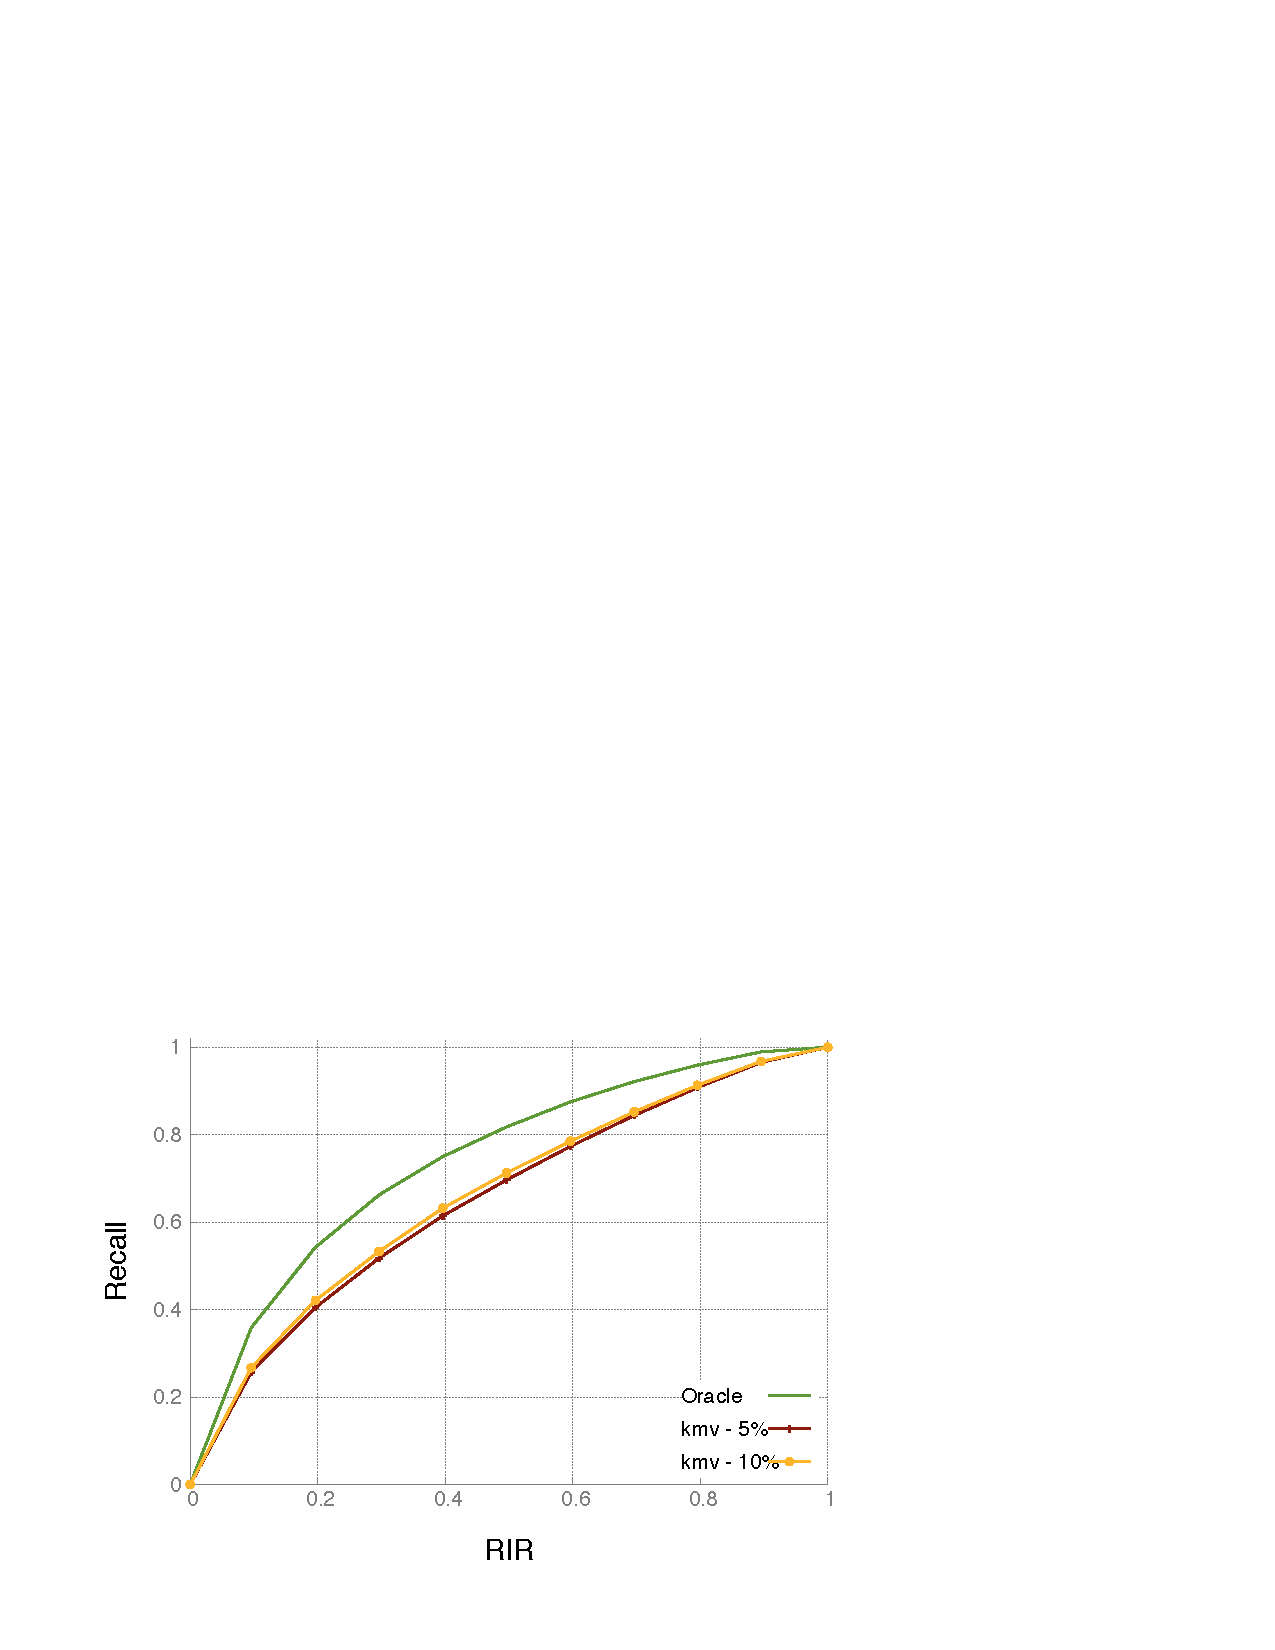
\includegraphics[width=0.60\textwidth]{plots/selection/cc_results/round2/pdf/wiki-varying-kmv-pse-7d.pdf}}
  \subfigure[UKGOV]{\label{fig:ukgov_vary_time_pse_fixed_7d}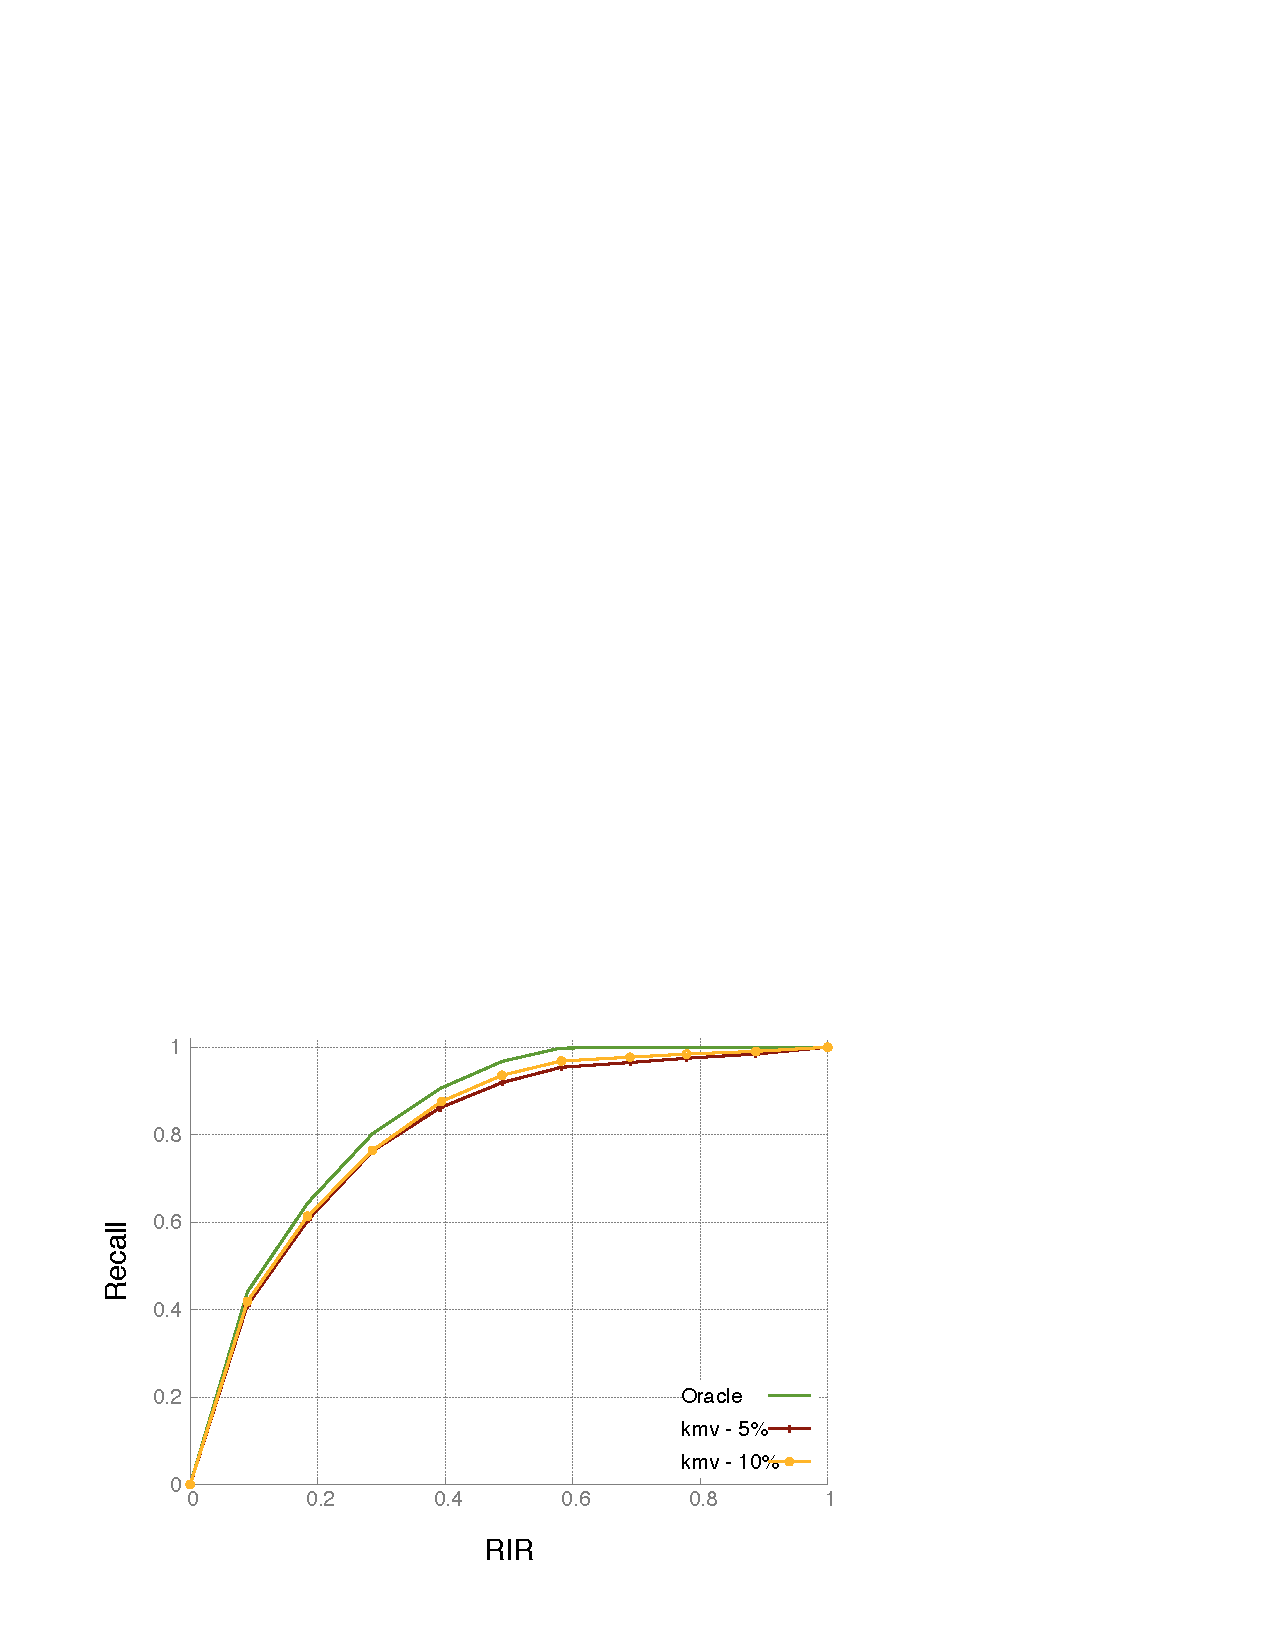
\includegraphics[width=0.60\textwidth]{plots/selection/cc_results/round2/pdf/ukgov-varying-kmv-pse-7d.pdf}}
  \subfigure[New York
  Times]{\label{fig:vary_time_nyt_psp_fixed_7d}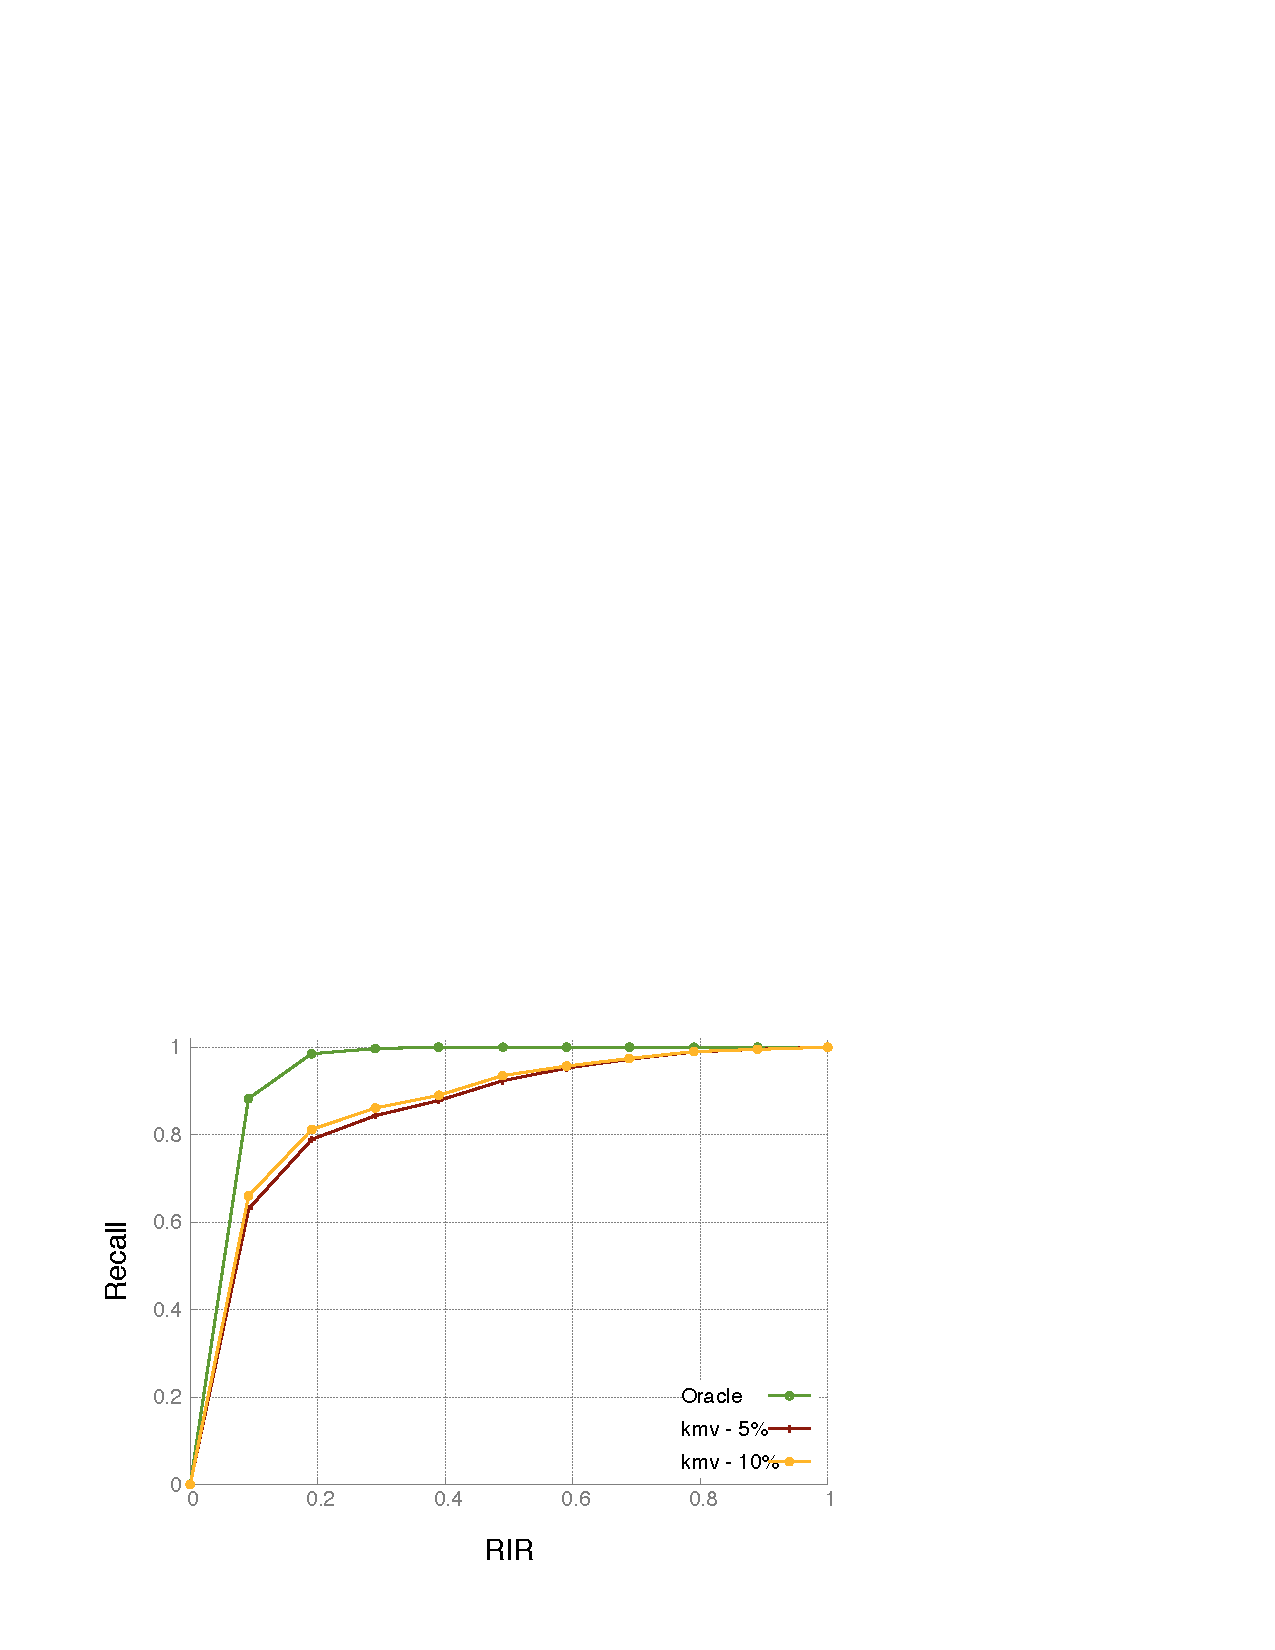
\includegraphics[width=0.60\textwidth]{plots/selection/cc_results/round2/pdf/nyt-varying-kmv-pse-7d.pdf}}
  
  \caption{Impact of using synopses }
  \label{fig:vary_kmv}
\end{figure*}

The next set of experiments is aimed at quantifying the impact of
using KMV synopses for the estimation of benefits and the effect of
different synopses size. For each dataset, we measure the average
recall obtained for each granularity of time-travel queries, using 5\%
and 10\% synopses, and compare them with those of 
\emph{oracle} outlined earlier. The results of this experiments over
indexes with \textbf{Fixed-7} partitioning, are shown in
Figure~\ref{fig:vary_kmv} for query-granularity of one year.

We can make the following observations from these plots: (i) The gap
between a 5\% KMV synopsis and 10\% synopsis is negligible,
prompting our choice of using 5\% KMV synopsis. (ii) Although oracle-based estimates are, as expected, better overall, improvements over
using KMV synopsis estimates are not significantly large. 

KMV synopsis are stored as arrays of doubles and much smaller than individual postings and can also be compressed and kept in memory. 
We also see from our experiments that query optimization using partition selection is a small fraction of the overall query-processing time. Thus, with a small memory footprint, and a quick estimation capability, we perceive that the use of KMV synopsis is a reasonable choice for partition selection. We used KMV-5\% in all our experiments unless explicitly mentioned. 

% These results also provide a first glimpse of the effectiveness of the
% partition selection methods themselves -- in the best case for NYT
% dataset, partition selection methods are able to answer with more than
% 80\% recall when the I/O budget is as small as 20\% of the RWOS.

\subsection {Impact of Partition Granularity}

\begin{figure*}
  \centering
  \subfigure[Wikipedia]{\label{fig:vary_time_wiki_psp_fixed_7d}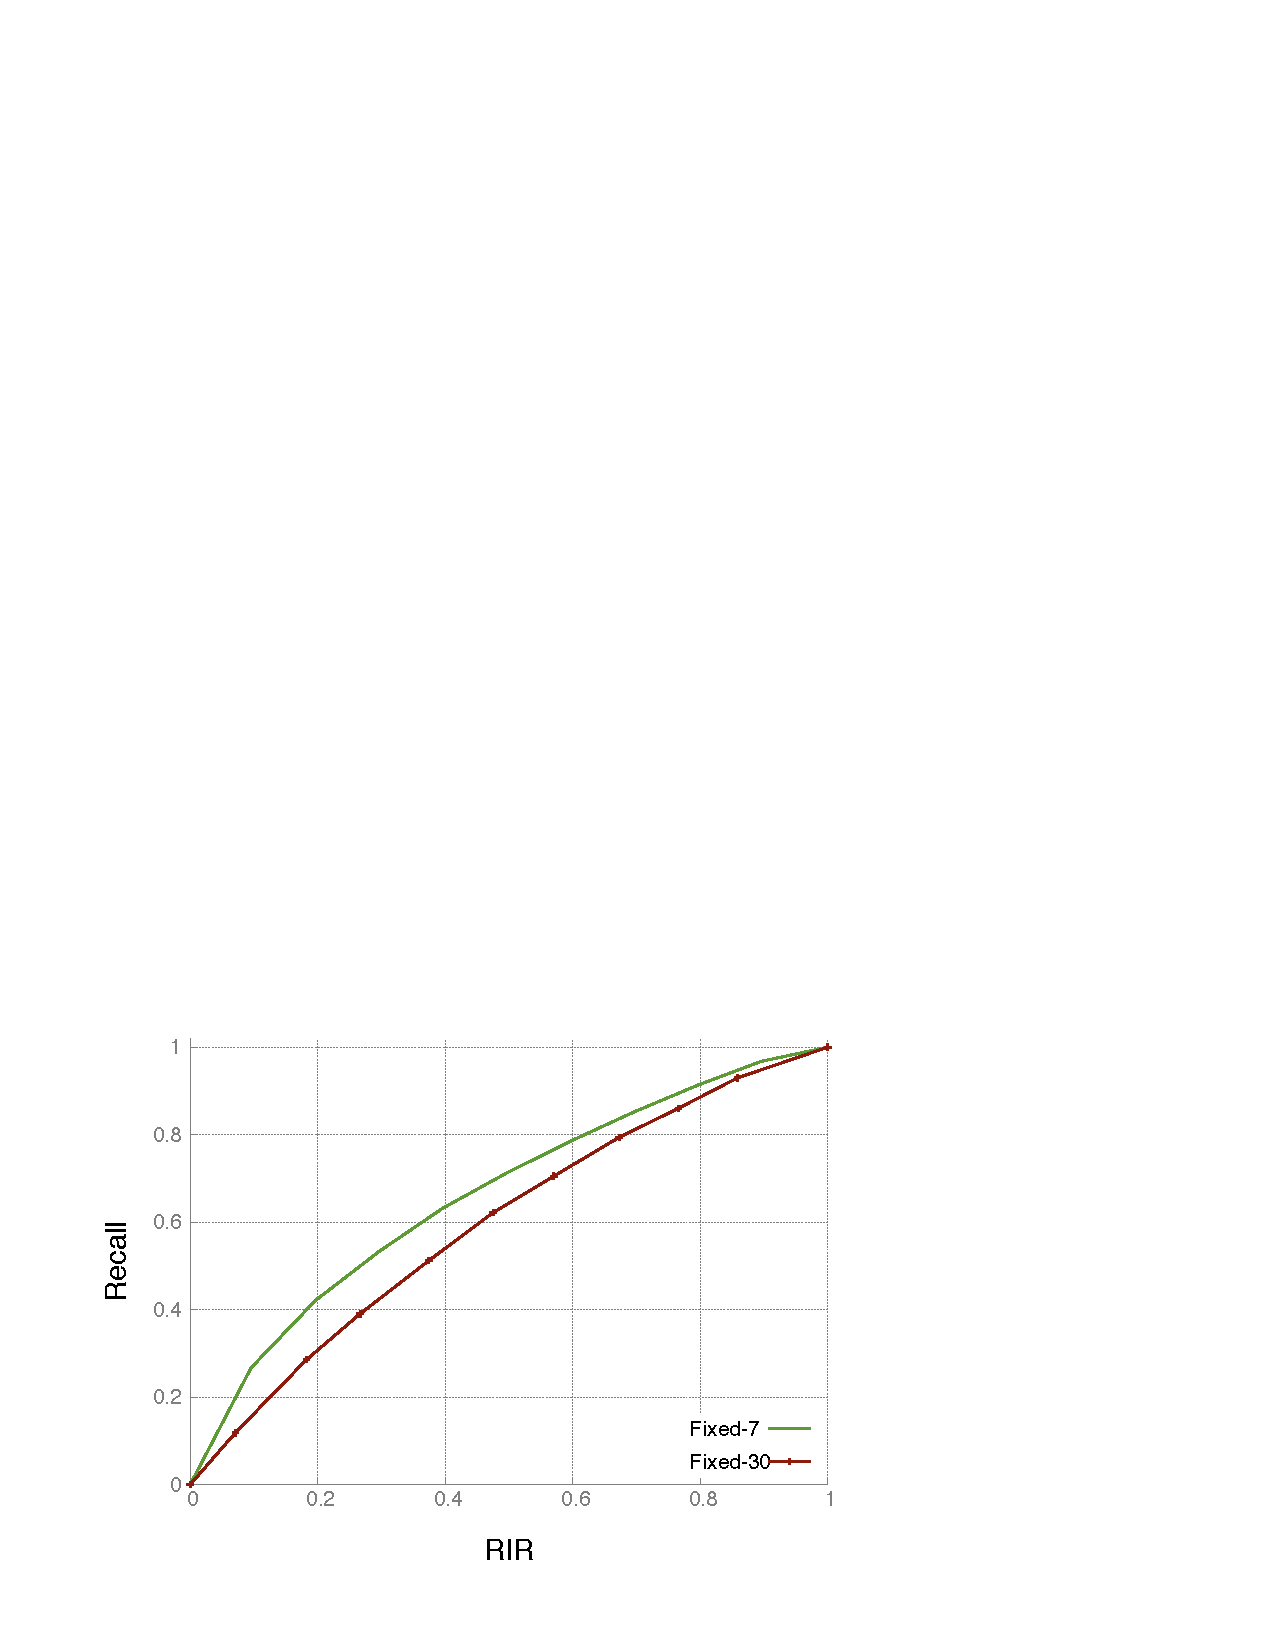
\includegraphics[width=0.60\textwidth]{plots/selection/cc_results/round2/pdf/wiki-partition-granularity-pse.pdf}}
  \subfigure[UKGOV]{\label{fig:vary_time_ukgov_psp_fixed_7d}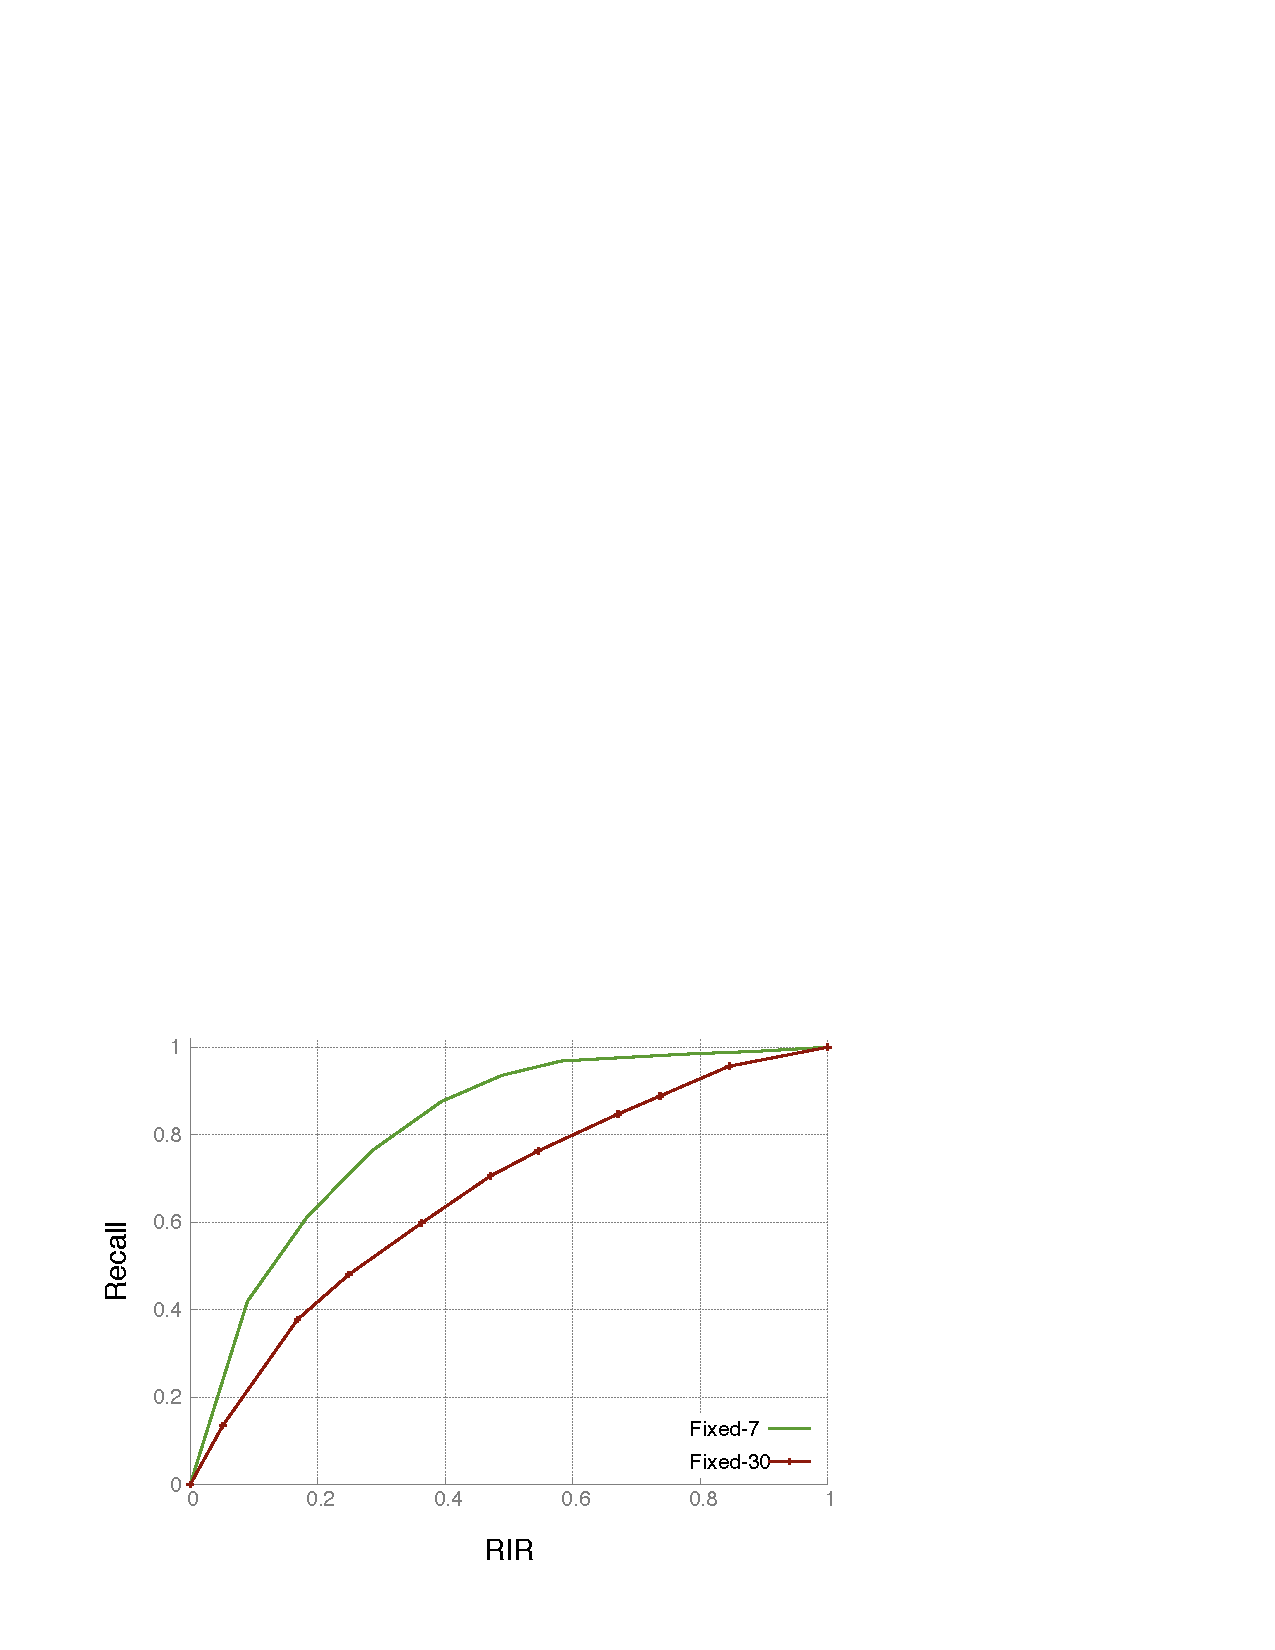
\includegraphics[width=0.60\textwidth]{plots/selection/cc_results/round2/pdf/ukgov-partition-granularity-pse.pdf}}
  \quad
  \subfigure[New York Times]{\label{fig:vary_time_nyt_psp_fixed_7d}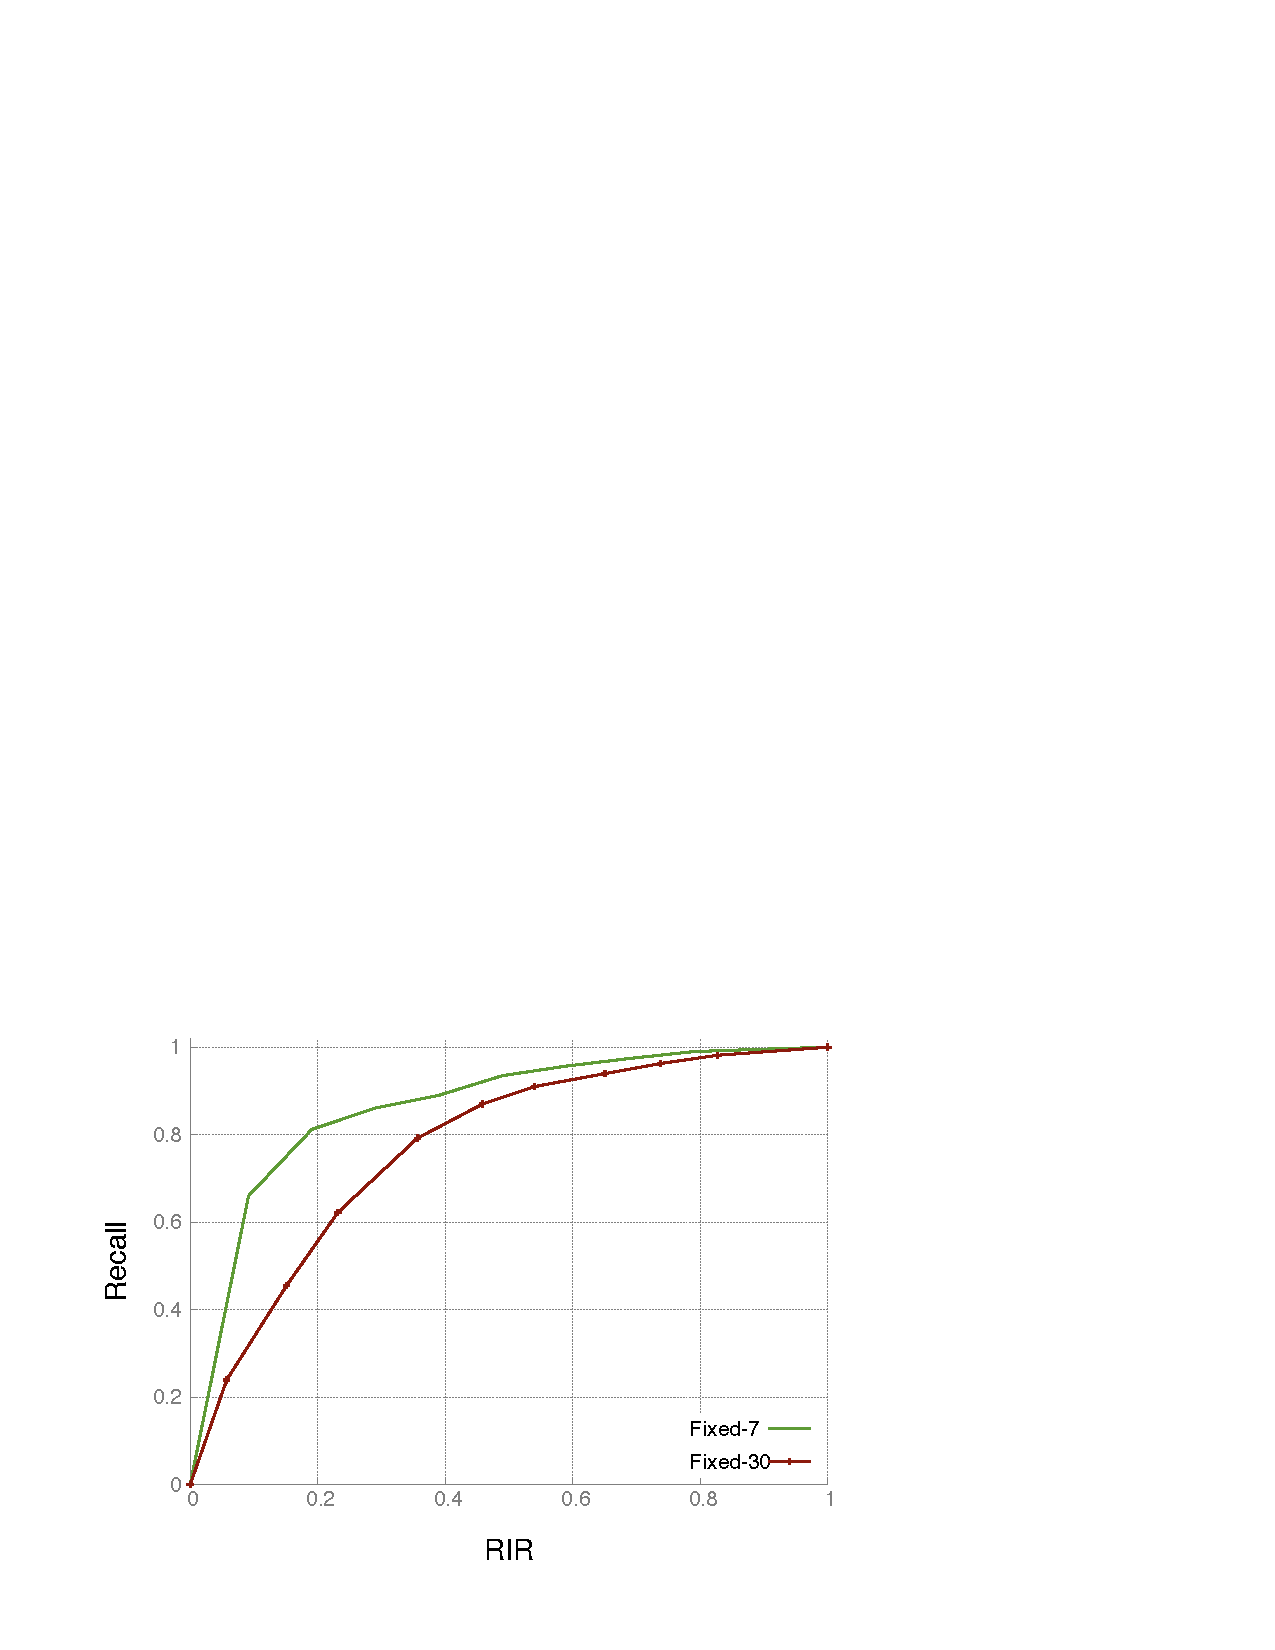
\includegraphics[width=0.60\textwidth]{plots/selection/cc_results/round2/pdf/nyt-partition-granularity-pse.pdf}}
  
  \caption{Effect of varying partition granularity on FIXED indexes }
  \label{fig:365day_part_gran}
\end{figure*}

\begin{figure*}
  \centering
  \subfigure[Wikipedia]{\label{fig:vary_time_wiki_pse_sb}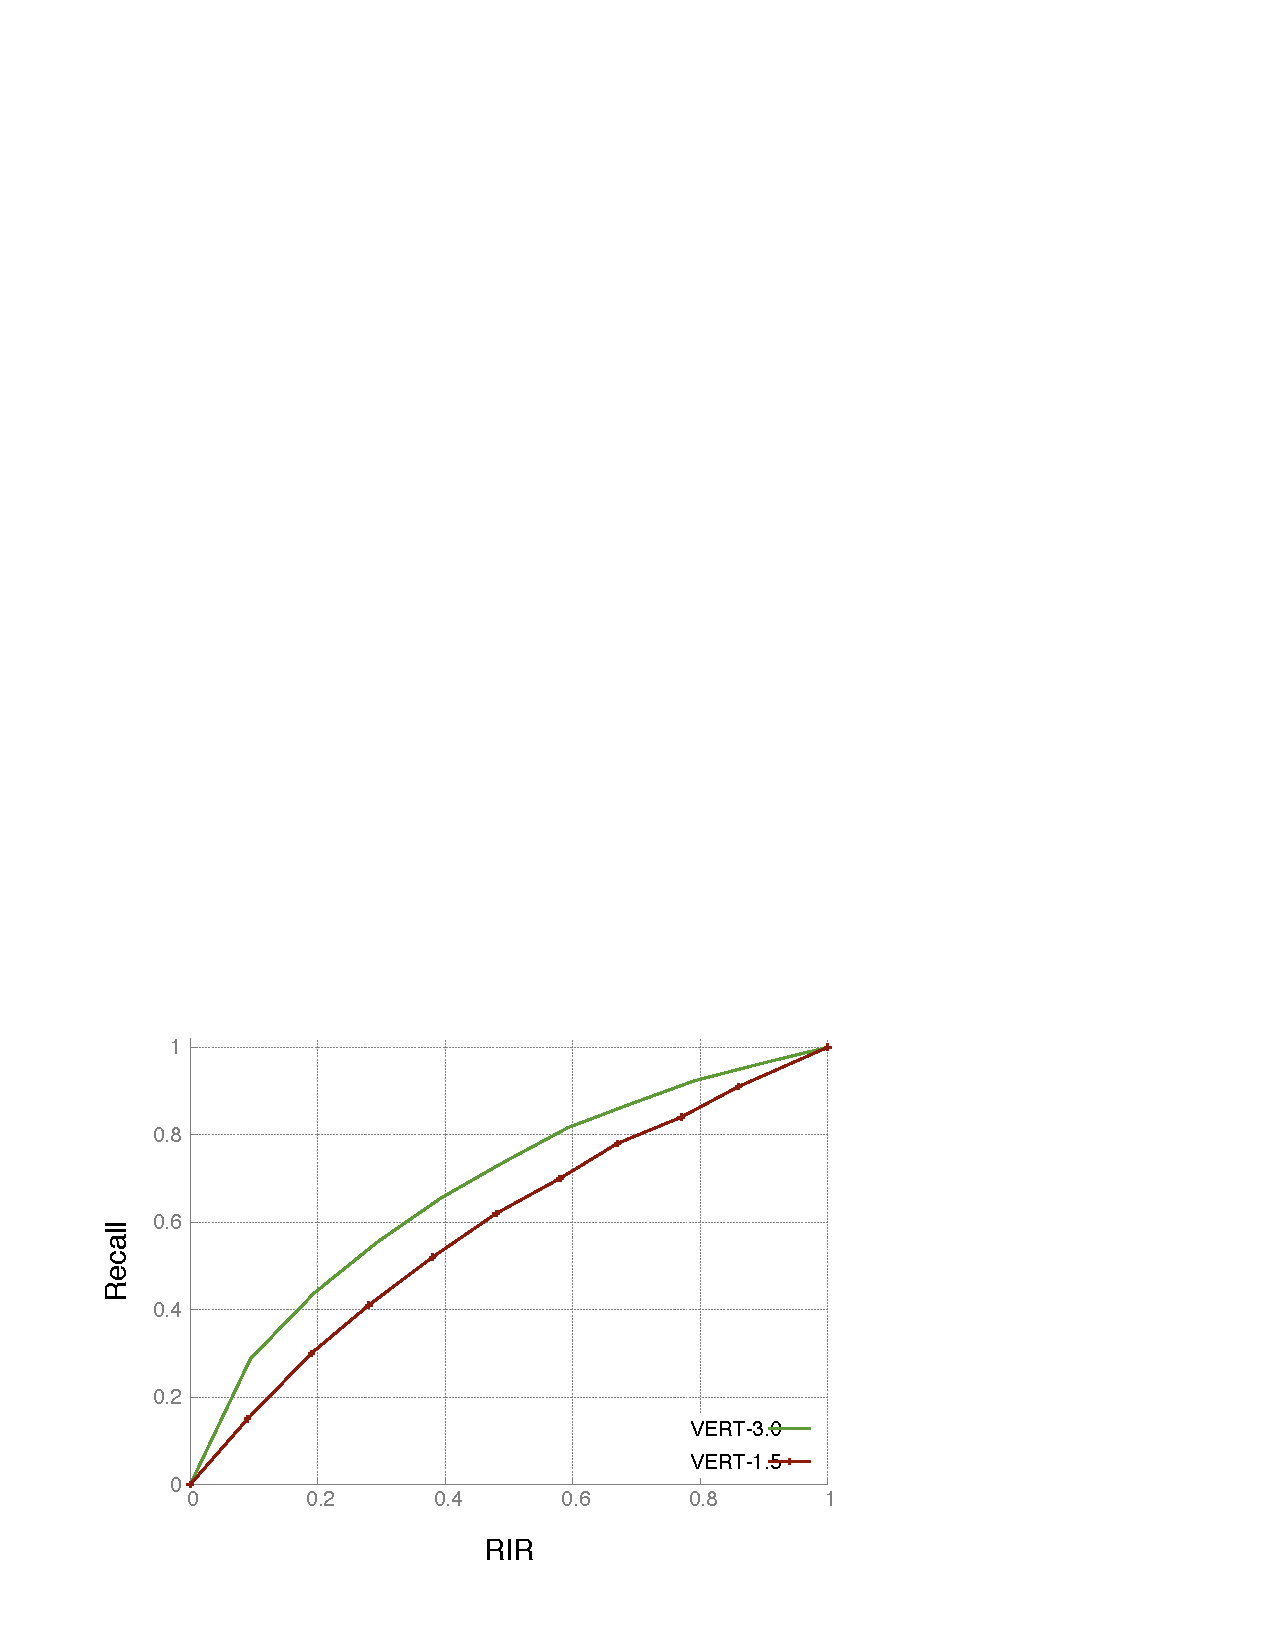
\includegraphics[width=0.60\textwidth]{plots/selection/cc_results/round2/pdf/wiki-partition-granularity-psp-sb.pdf}} 
  \subfigure[UKGOV]{\label{fig:vary_time_ukgov_pse_sb}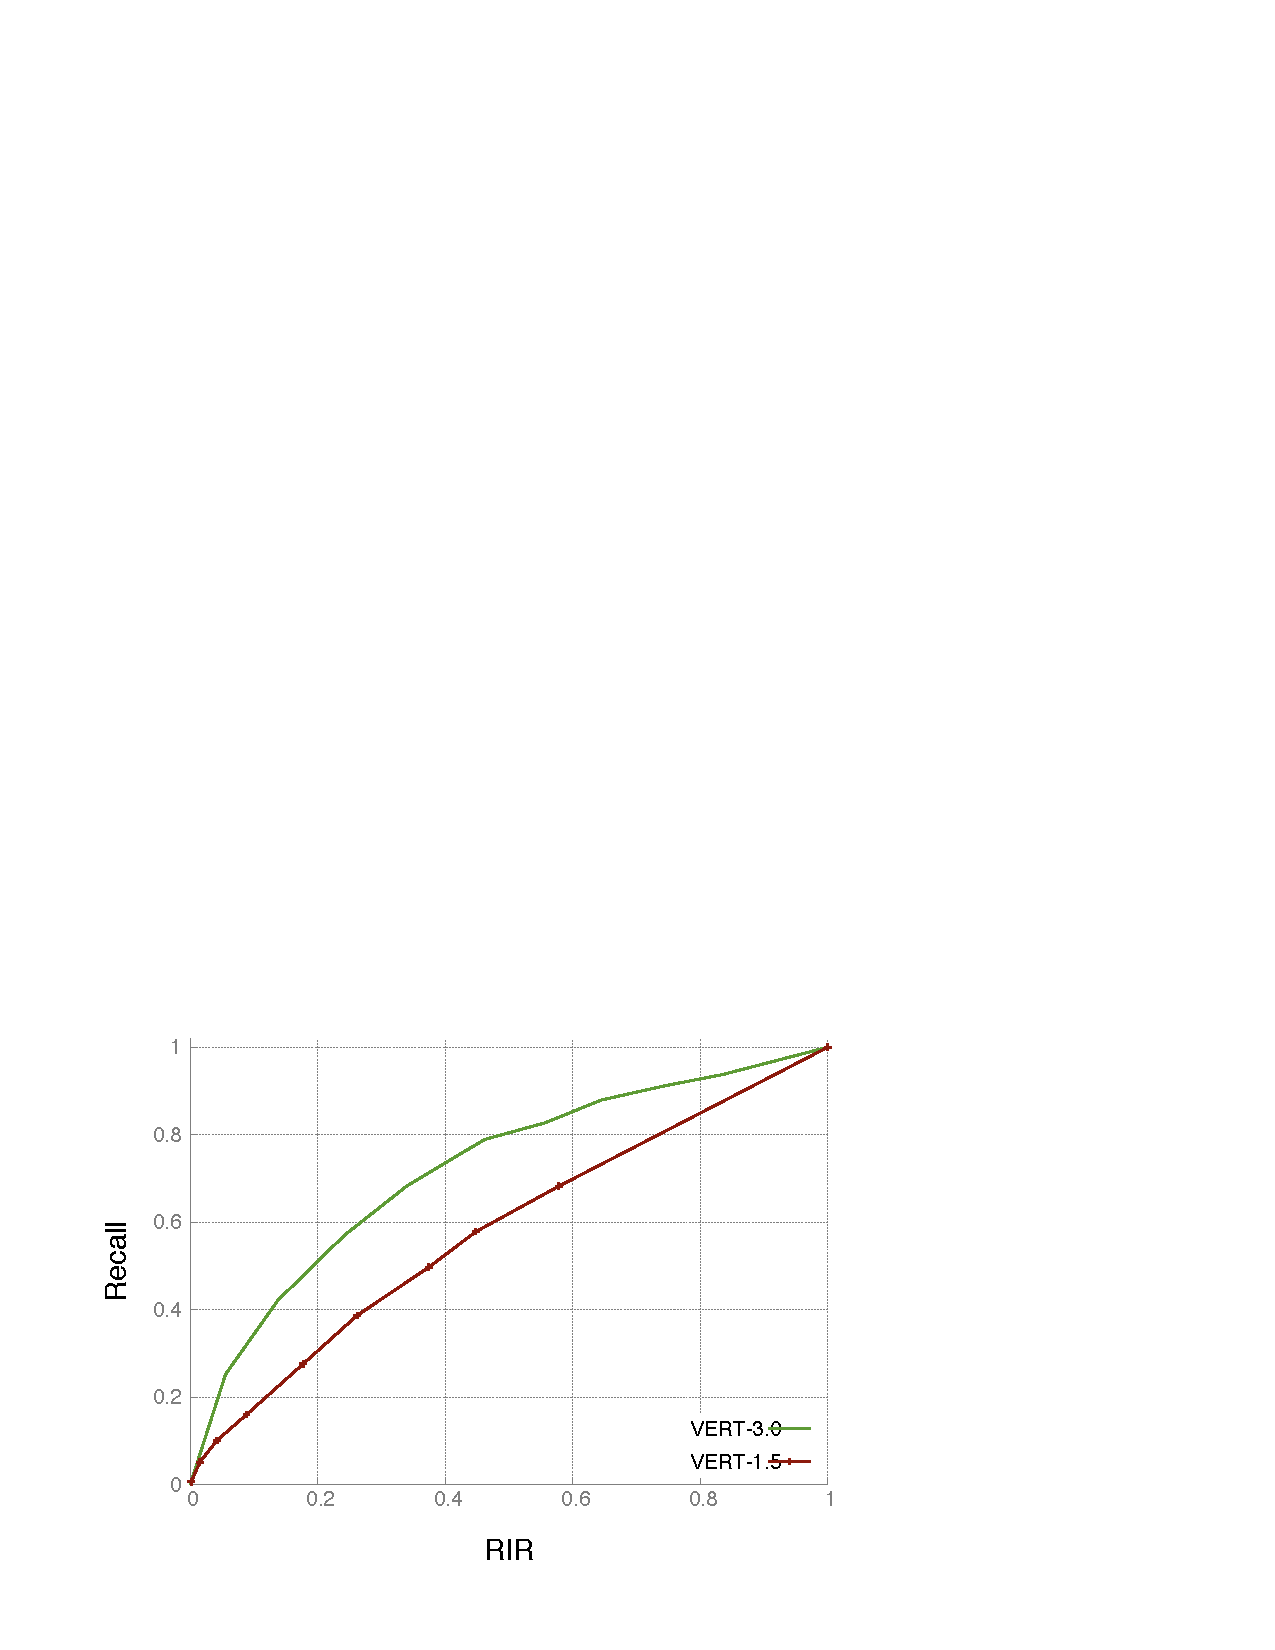
\includegraphics[width=0.60\textwidth]{plots/selection/cc_results/round2/pdf/ukgov-partition-granularity-psp-sb.pdf}}
  \subfigure[New York Times]{\label{fig:vary_time_nyt_pse_sb}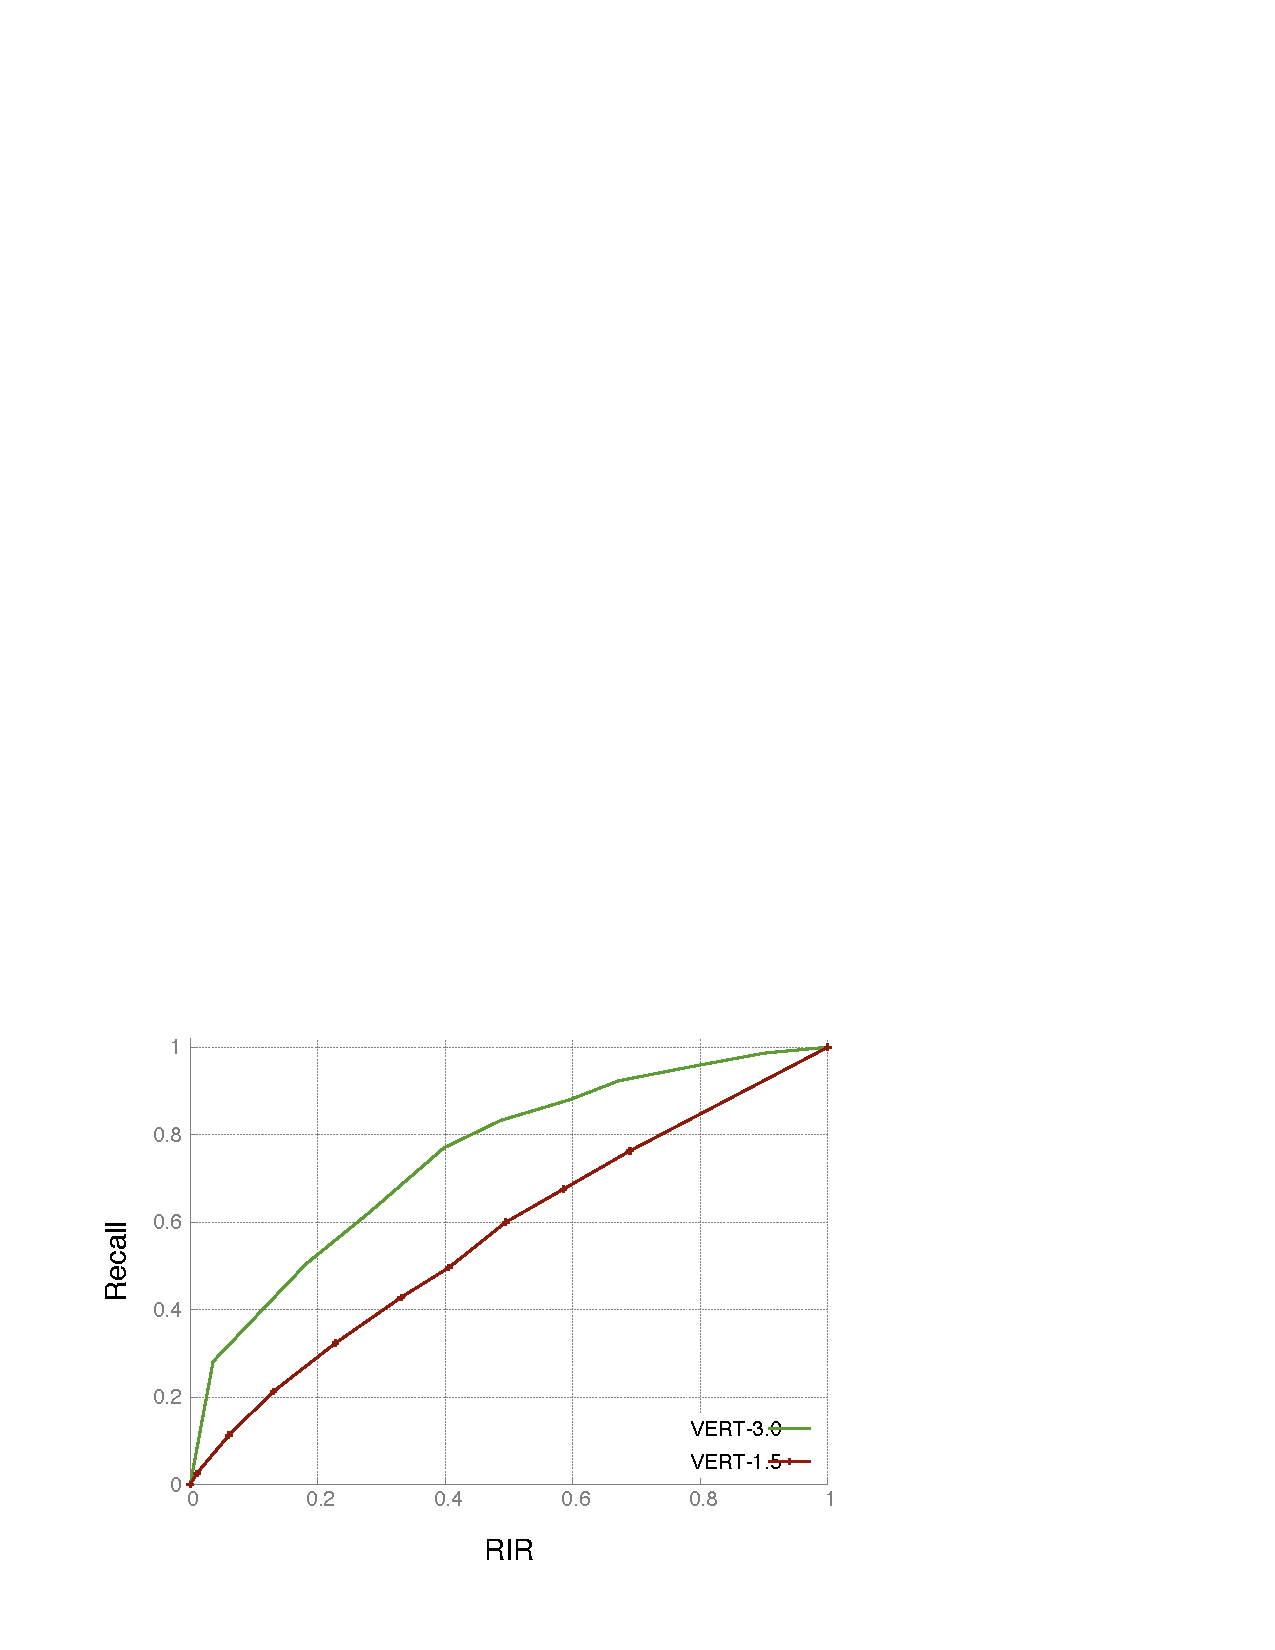
\includegraphics[width=0.60\textwidth]{plots/selection/cc_results/round2/pdf/nyt-partition-granularity-psp-sb.pdf}}
  
  \caption{Effect of varying partitioning granularities on VERT indexes}
  \label{fig:365day_part_gran_sb}
\end{figure*}

In our final experiment, we wanted to examine the effect of partition selection over varying partitioning granularities. We experimented with two different granularities of fixed partitioning --
7-day and 30-day time-intervals, resulting in \textbf{Fixed-7} and \textbf{Fixed-30}
index configurations. \textbf{Fixed-7} has a higher number of partitions,
thus can be seen as having smaller partition sizes in comparison to
\textbf{Fixed-30}. Clearly, this allows efficient processing of time-point
or short duration queries. However, it deteriorates for larger
time-interval queries if partition selection is not employed. On the other hand, performance with partition selection shown in
Figure~\ref{fig:365day_part_gran} for year-granularity queries,
shows that even for smaller partitions sizes this issue can be
effectively alleviated. 

We also considered the partitions created by vertical partitioning of granularities --- VERT-1.5 and VERT-3.0. We see a similar effect as in the case of fixed partitioning, i.e., selection is much more effective for partitioning schemes with high replication of postings. In this case, selection over VERT-3.0 provides higher benefit consistently over VERT-1.5 (see Figure~\ref{fig:365day_part_gran_sb}). 

\section{Related Work}
\label{chap:selection:relwork}

Closest to the ideas presented here is the work on
time-travel text search~\cite{kberberi:sigir2007} that allows users to
search only the part of a document collection that existed at a given
time point. To support this functionality efficiently, posting lists
from an inverted index are temporally partitioned either according to
a given space bound or required performance guarantee. Postings whose
valid-time interval overlaps with multiple of the determined temporal
partitions are judiciously replicated and put into multiple posting
lists, thus increasing the overall size of the index.

% Temporal Databases
Join-processing techniques for temporal databases~\cite{Gao2005} are a
second class of related work whose focus, to the best of our
knowledge, has been on producing accurate query results opposed to the
approximate results that our techniques deliver.

% Approximate Query Processing
As data volumes grow, many queries are increasingly expensive to
evaluate accurately. However, an approximate but almost accurate
answer that is delivered quickly is often good enough. Approximate
query processing techniques~\cite{Acharya1999,Acharya1999a} developed
by the database community aim at quickly determining an approximate
answer and, to this end, typically leverage data statistics (often
approximated using histograms), sampling, and other data synopses. In
contrast to our scenario, approximate query processing techniques
target scenarios with a well-designed relational schema that implies
certain reasonable queries (e.g., based on foreign keys). When cast
into a relational schema, our scenario gives rise to millions of
relations (corresponding to terms and their corresponding
partitions).


\section{Summary}
\label{chap:selection:sec:summary}
In this chapter, we present a framework for efficient approximate processing of keyword queries over a temporally-partitioned inverted index. By using a small synopsis for each partition we identify partitions that maximize the number of final non-redundant results and schedule them for processing early on. Our approach aims to maximize  the recall at each stage of query execution given budget on the index-access cost.

Our experimental evaluation shows that our proposed methods can
compute more than 80\% of final results even when the I/O budget is
set as low as 50\% of the total size of the partitions that satisfy
the temporal predicate. We derive the following insights from our experimental results. Firstly, the choice of the selection methods does not seem to affect the results. Both selection methods are able to deliver a relatively high recall by accessing a small fraction of the index. Secondly, our model for expected query processing time depending on the access costs is vindicated as the wall-clock times seem to be correlated with the fraction of the index accessed. Finally, selection methods are more effective for fine-granular indexes.



